%%%%%%%%%%%%%%%%%%%%%%%%%%%%%%%%%%%%%%%%%%%%%%%%%%%%%%%%%%%%%%%%%%%%%%%%%%%%%%%%%%
%%%%%%%%%%%%%%%%%%%%%%%%%%%%%%%%%%%%%%%%%%%%%%%%%%%%%%%%%%%%%%%%%%%%%%%%%%%%%%%%%%
%% Adapted from Gilles Castel's work: https://github.com/gillescastel/masterthesis 
%%%%%%%%%%%%%%%%%%%%%%%%%%%%%%%%%%%%%%%%%%%%%%%%%%%%%%%%%%%%%%%%%%%%%%%%%%%%%%%%%%
%%%%%%%%%%%%%%%%%%%%%%%%%%%%%%%%%%%%%%%%%%%%%%%%%%%%%%%%%%%%%%%%%%%%%%%%%%%%%%%%%%
\documentclass[working]{tuftebook}

\usepackage[utf8]{inputenc}
\usepackage[T1]{fontenc}
\usepackage{textcomp}

\usepackage{url}
\usepackage[mode=buildnew]{standalone} % to include tikz figs precompiled
\usepackage{eucal} %mathscr like \mathcal{}
\usepackage[ruled,vlined]{algorithm2e}
\usepackage{mathtools}


\RequirePackage[style=authoryear,
	backend=biber,
	natbib=true,
	maxcitenames=2,
	mincitenames=1,
	dashed=false,
	isbn=false,
	url=false,
	eprint=false,
	doi=false,
	uniquelist=minyear % prevent issue for references of the same first author (even in different years)
]{biblatex}
\addbibresource{bibliography.bib} % The filename of the bibliography

\usepackage[autostyle=true]{csquotes} % Required to generate language-dependent quotes in the bibliography

\usepackage{hyperref}
\hypersetup{
	colorlinks=true,
	linkcolor=blue,
	filecolor=magenta,
	urlcolor=magenta,
	citecolor=blue,
}
\usepackage[noabbrev]{cleveref}

% Adds Bibliography, ... to Table of Contents
\usepackage[nottoc]{tocbibind}

\usepackage{graphicx}
\usepackage{float}
\usepackage[usenames,dvipsnames,svgnames]{xcolor}

% \usepackage{cmbright}

\usepackage{amsmath, amsfonts, mathtools, amsthm, amssymb}
\usepackage{mathrsfs}
\usepackage{cancel}


\usepackage{tikz}
\usepackage{tikz-cd}

% theorems
\usepackage{setup/theorems}

\makeatother

% figure support (https://castel.dev/post/lecture-notes-2)
\usepackage{import}
\usepackage{xifthen}
\pdfminorversion=7
\usepackage{pdfpages}
\usepackage{transparent}


\makeatletter
\newif\ifworking
\@ifclasswith{tuftebook}{working}{\workingtrue}{\workingfalse}
\makeatother

\newcommand{\incfig}[2][1]{%
	% \ifworking{\makebox[0pt][c]{\color{gray}{\scriptsize\textsf{#2}}}}\fi%
	\def\svgwidth{#1\textwidth}
	\import{./figures/}{#2.pdf_tex}
}

\newcommand{\fullwidthincfig}[2][0.90]{%
	% \ifworking{\makebox[0pt][l]{\color{gray}{\scriptsize\textsf{#2}}}}\fi%
	\def\svgwidth{#1\paperwidth}
	\import{./figures/}{#2.pdf_tex}
}


\newcommand{\minifig}[2]{%
	\def\svgwidth{#1}%
	\begingroup%
	\setbox0=\hbox{\import{./figures/}{#2.pdf_tex}}%
	\parbox{\wd0}{\box0}\endgroup%
	\hspace*{0.2cm}
}

% %http://tex.stackexchange.com/questions/76273/multiple-pdfs-with-page-group-included-in-a-single-page-warning
\pdfsuppresswarningpagegroup=1

\newcommand\todo[1]{\ifworking {{\color{red}{#1}}} \else {}\fi}
\newcommand\charlotte[1]{\ifworking {{\color{blue}{#1}}} \else {}\fi}

\author{Niccolò Zanotti}


\usepackage{multirow}
\def\block(#1,#2)#3{\multicolumn{#2}{c}{\multirow{#1}{*}{$ #3 $}}}

% \overfullrule=1mm

\newenvironment{myproof}[1][\proofname]{%
	\proof[\rm \bf #1]%
}{\endproof}

%----------------------------------------------------------------------------------------
%	USER DEFINED COMMANDS
%----------------------------------------------------------------------------------------

\usepackage{xparse}
\usepackage{siunitx}
\usepackage{bm}


%%%%%%%%%%%%%%%%%%%%%%%%%%%%%%%%%%%%%%%%%%%%%%%%%%%%
%%%%%%%%%%%%%%%%% MATHEMATICAL %%%%%%%%%%%%%%%%%%%%%
%%%%%%%%%%%%%%%%%%%%%%%%%%%%%%%%%%%%%%%%%%%%%%%%%%%%
\newcommand\N{\ensuremath{\mathbb{N}}}
\newcommand\R{\ensuremath{\mathbb{R}}}
\newcommand\Z{\ensuremath{\mathbb{Z}}}
\renewcommand\O{\ensuremath{\emptyset}}
\newcommand\Q{\ensuremath{\mathbb{Q}}}
\newcommand\C{\ensuremath{\mathbb{C}}}
\let\implies\Rightarrow
\let\impliedby\Leftarrow
\let\iff\Leftrightarrow

%%% Commands specific to THEORY OF COMPUTATION notes
\newcommand\enc[1]{\ensuremath{\llcorner #1 \lrcorner}}
% https://en.wikipedia.org/wiki/Floor_and_ceiling_functions
\newcommand\floor[1]{\ensuremath{\lfloor #1 \rfloor}}
\newcommand\ceil[1]{\ensuremath{\lceil #1 \rceil}}
\newcommand\oneton[1]{\ensuremath{[ #1 ]}} % [n] = {1, ..., n}
\newcommand\indist[1]{\ensuremath{\in_{\scriptscriptstyle\text{R}}} #1}  % distrubuted randomly according to 
\newcommand\binstrings{\ensuremath{\{ 0,1 \}^* }}
\newcommand\binset{\ensuremath{\{ 0,1 \} }}
\newcommand\lang[1]{\ensuremath{\mathcal{#1}}} % language notation
\newcommand\strlen[1]{\ensuremath{\left \lvert #1 \right \rvert}} %lenght of a binary string
\newcommand\blank{\ensuremath{\square}}
\newcommand\start{\ensuremath{\rhd}}
\newcommand{\fail}{\bm{\times}}
\newcommand{\success}{\checkmark}
\renewcommand{\epsilon}{\varepsilon}
\newcommand\karpred{\ensuremath{\leq_p}} % karp-reducible
\newcommand{\HALT}{\ifmmode\mathtt{HALT}\else\texttt{HALT}\fi}
\newcommand{\UC}{\ifmmode\mathtt{UC}\else\texttt{UC}\fi}
\newcommand{\DTIME}{\textbf{DTIME}}
\newcommand{\FDTIME}{\textbf{FDTIME}}
\newcommand{\NTIME}{\textbf{NTIME}}
\renewcommand{\P}{\textbf{P}}
\newcommand{\NP}{\textbf{NP}}
\newcommand{\EXP}{\textbf{EXP}}
\newcommand{\FEXP}{\textbf{FEXP}}
\newcommand{\FP}{\textbf{FP}}
\newcommand{\SAT}{\ifmmode\mathtt{SAT}\else\texttt{SAT}\fi}
\newcommand{\kSAT}[1]{\ifmmode\mathtt{#1SAT}\else\texttt{#1SAT}\fi}
\newcommand{\INDSET}{\ifmmode\mathtt{INDSET}\else\texttt{INDSET}\fi}
\newcommand{\CLIQUE}{\ifmmode\mathtt{CLIQUE}\else\texttt{CLIQUE}\fi}
\newcommand{\kCLIQUE}[1]{\ifmmode\mathtt{#1CLIQUE}\else\texttt{#1CLIQUE}\fi}
\newcommand{\COL}{\ifmmode\mathtt{COL}\else\texttt{COL}\fi}
\newcommand{\kCOL}[1]{\ifmmode\mathtt{#1 COL}\else\texttt{#1 COL}\fi}
\newcommand{\SUBSETSUM}{\ifmmode\mathtt{SUBSETSUM}\else\texttt{SUBSETSUM}\fi}
\newcommand{\NODECOVER}{\ifmmode\mathtt{NODECOVER}\else\texttt{NODECOVER}\fi}



\newcommand{\dx}{\,\mathrm{d}\bm{x}}
\newcommand{\dt}{\,\mathrm{d}t}
\newcommand{\dxOne}{\,\mathrm{d}x}
\newcommand{\dhOne}{ \,\mathrm{d}h}
\newcommand{\dS}{\,\mathrm{d}S}
\newcommand{\totalt}{\frac{\mathrm{d}}{\mathrm{dt}}}
\newcommand{\totald}[2]{\frac{\mathrm{d}#1}{\mathrm{d}#2}}
\newcommand{\timed}[1]{\frac{\mathrm{d} #1}{\mathrm{d}t}}
\newcommand{\partialt}[1]{\frac{\partial #1}{\partial t}}
\newcommand{\partialphi}[1]{\frac{\partial #1}{\partial \phi}}
\newcommand{\partiallambda}[1]{\frac{\partial #1}{\partial \lambda}}
\newcommand{\partialx}[1]{\frac{\partial #1}{\partial x}}
\newcommand{\partialy}[1]{\frac{\partial #1}{\partial y}}
\newcommand{\partialz}[1]{\frac{\partial #1}{\partial z}}
\newcommand{\materiald}[1]{\frac{\mathrm{D} #1}{\mathrm{D}t}}
\newcommand{\objmateteriald}[1]{\frac{\mathcal{D} #1}{\mathcal{D}t}}
\newcommand{\flux}{\mathcal{F}}
\newcommand{\jump}[1]{ \{\{#1\}\} }
\newcommand{\avg}[1]{ [[#1]] }
\newcommand{\eq}[1]{Equation~#1}
\newcommand{\timemean}[1]{\overline{#1}} %time mean
\newcommand{\zonmean}[1]{[#1]} %zonal mean
\newcommand{\fig}[1]{Figure~#1}
\newcommand{\secref}[1]{Section~#1}
\newcommand{\chapref}[1]{Chapter~#1}
\newcommand{\tabref}[1]{Table~#1}
\newcommand{\mat}[1]{\mathbf{#1}}      % matrix
\newcommand{\tens}[2]{\mat{#1}:#2}     % tensor

% Vector calculus
\renewcommand{\vec}[1]{\ifmmode\bm{#1}\else\ensuremath{\bm{#1}}\fi} %vector
\newcommand{\unitv}[1]{\bm{\hat{#1}}}  % unit vector
\newcommand{\grad}[1]{\bm{\nabla} #1}
\newcommand{\curl}[1]{\bm{\nabla} \times #1}
\newcommand{\diverg}[1]{\bm{\nabla} \cdot #1}
%%%%%%%%%%%%%%%%%%%%%%%%%%%%%%%%%%%%%%%%%%%%%%%%%%%%
%%%%%%%%%%%%%%%%%%%% SIUNITX %%%%%%%%%%%%%%%%%%%%%%%
%%%%%%%%%%%%%%%%%%%%%%%%%%%%%%%%%%%%%%%%%%%%%%%%%%%%
\DeclareSIUnit[quantity-product = \,]{\psu}{psu}
\newcommand{\qtyranged}[3]{\qtyrange[range-phrase = {--}]{#1}{#2}{#3}} % \qtyranged{<left range>}{<right range>}{<unit>}, e.g. 1-2 km

%%%%%%%%%%%%%%%%%%%%%%%%%%%%%%%%%%%%%%%%%%%%%%%%%%%%
%%%%%%%%%%%%%%%%%% SOURCE FILES %%%%%%%%%%%%%%%%%%%%
%%%%%%%%%%%%%%%%%%%%%%%%%%%%%%%%%%%%%%%%%%%%%%%%%%%%
% \newcommand{\chapterX}{\href{https://github.com/niccolozanotti/repo-name/blob/main/chapters/chapterX.tex}{chapterX.tex}}

%%%%%%%%%%%%%%%%%%%%%%%%%%%%%%%%%%%%%%%%%%%%%%%%%%%%
%%%%%%%%%%%%%%%%%%%% MISCELLANEA %%%%%%%%%%%%%%%%%%%
%%%%%%%%%%%%%%%%%%%%%%%%%%%%%%%%%%%%%%%%%%%%%%%%%%%%


\usepackage{enumitem}
\newlist{abbrv}{itemize}{1}
\setlist[abbrv,1]{label=,labelwidth=1in,align=parleft,itemsep=0.1\baselineskip,leftmargin=!}

\DeclareMathOperator{\Crit}{Crit}
\newcommand{\Cinfty}{C^\infty}

\newcommand{\stable}[1]{W^s(#1)}
\newcommand{\unstable}[1]{W^u(#1)}
\newcommand{\unstableb}[1]{\overline{W}^u(#1)}

\def\symbolentry#1#2#3{\item[#2] #3}
\def\sort#1{}

\makeatletter
\newcommand{\superimpose}[2]{%
	{\ooalign{$#1\@firstoftwo#2$\cr\hfil$#1\@secondoftwo#2$\hfil\cr}}}
\makeatother

% https://tex.stackexchange.com/questions/134863/command-for-transverse-and-not-pitchfork-as-used-in-guillemin-and-pollack
% \newcommand{\tcap}{\mathrel{\mathpalette\superimpose{{\raise0.15ex\hbox{$\top$}}{\cap}}}}
\newcommand{\tcap}{\pitchfork}

\newcommand\traj[2]{\mathcal M(#1, #2)}
\renewcommand\L[2]{\mathcal L(#1, #2)}
\newcommand\Lb[2]{\overline{\mathcal L}(#1, #2)}

\newcommand\nX[3]{n_{#1}(#2, #3)}
\newcommand\NX[3]{N_{#1}(#2, #3)}
\newcommand\HM[3][]{HM_{#1}(C_\bul(#2), \partial_#3)}
\newcommand\HMf[2][]{HM_{#1}(#2)}

\DeclareMathOperator{\Ind}{Ind}
\DeclareMathOperator{\Rank}{Rank}

\DeclareMathOperator{\codim}{codim}
% \DeclareMathOperator{\grad}{grad}

\DeclareMathOperator{\Ker}{Ker}
\renewcommand{\Im}{\operatorname{Im}}

\newcommand\sphere[1]{S^{#1}}
\newcommand\cdisk[1]{B^{#1}}
\newcommand\odisk[1]{D^{#1}}
\newcommand\bul{\bullet}


\DeclareMathOperator{\Hom}{Hom}

\newcommand{\listofsymbols}{
	\chapter*{List of symbols}
	\begin{abbrv}

		%        \symbolentry{0}{$M \tcap N$}{Transverse intersection}
		%        \symbolentry{1}{$\left<\cdot ,\cdot  \right>$}{Riemannian metric on a manifold or,\\ Inner product on space of critical points $\left<c, d \right> = \delta_{cd}$}
		%        \symbolentry{2}{$N \cdot N'$}{Intersection number of two manifolds}
		%        \symbolentry{A}{$A$}{A $\Z$-module, i.e.\ an abelian group}
		%        \symbolentry{B}{$\cdisk{n}$}{Closed disk of dimension $n$}
		%        \symbolentry{Ck}{$C_k(f, \Z)$}{
		%        Free module over $\Z$ generated by index $k$ critical points of $f$, i.e.\ the space of formal sums of index $k$ critical points
		%    }
		%        \symbolentry{Ck}{$C_k(f, \Z_2)$}{Vector space over $\Z_2$ generated by the index $k$ critical points of the Morse function $f$}
		%        \symbolentry{Codim}{$\codim N$}{Codimension of $N$}
		%        \symbolentry{Codim}{$\dim N$}{Dimension of $N$}
		%        \symbolentry{Critk}{$\Crit_k f$}{Critical points of $f$ of index $k$}
		%        \symbolentry{Crit}{$\Crit f$}{Critical points of $f$}
		%        \symbolentry{C}{$\Cinfty(M, N)$}{Smooth maps from $M$ to  $N$}
		%        \symbolentry{DpartialA}{$\partial_{X, k}$}{Morse differential associated to pseudo-gradient $X$}
		%    \symbolentry{DpartialM}{\mbox{$[\partial_k]$}}{Matrix of the Morse differential $\partial_k: C_k \to  C_{k-1}$}
		%        \symbolentry{D}{$\odisk{n}$}{Open disk of dimension $n$}
		%        \symbolentry{Grad}{$\grad f$}{Gradient of  $f$, i.e.\ $(df)^{\sharp}$}
		%        \symbolentry{HM2}{$\HMf{M; \Z_2}$}{Morse homology of a manifold $M$ with coefficients in $\Z_2$}
		%        \symbolentry{HM3}{$\HMf{M; \Z}$}{Morse homology of a manifold $M$ with coefficients in $\Z$}
		%        \symbolentry{HM}{$\HM{f}{X}$}{\mbox{Morse homology of Morse function $f$ and pseudo-gradient $X$}}
		%        \symbolentry{H}{$H_k(M, N)$}{Singular homology of $M$ relative to $N$}
		%        \symbolentry{H}{$H_k(M; \Z)$}{Singular homology of $M$ over $\Z$}
		%        \symbolentry{H}{$H_k(M; \Z_2)$}{Singular homology $M$ over $\Z_2$}
		%        \symbolentry{Ind}{$\Ind a$}{Index of critical point $a$}
		%        \symbolentry{La}{$\L{p}{q}$}{Moduli space of unbroken trajectories between $p$ and $q$, i.e.\ $\traj{p}{q} / \R$, where $\R$ acts by time translations}
		%        \symbolentry{Lb}{$\Lb{p}{q}$}{Space of broken and unbroken trajectories between $p$ and $q$, the compactification of $\L pq$}
		%        \symbolentry{M}{$M$}{A smooth manifold}
		%        \symbolentry{M}{$\traj{p}{q}$}{Set of all points on trajectories following a pseudo-gradient from $p$ to $q$, $\unstable p \tcap \stable q$}
		%        \symbolentry{NX}{$\NX{X}{p}{q}$}{Signed number of trajectories of $X$ connecting  $p$ to $q$}
		%        \symbolentry{NX}{$\nX{X}{p}{q}$}{Number of trajectories of $X$ connecting  $p$ to $q$}
		%        \symbolentry{Pi}{$\pi_k(M)$}{Homotopy group of a manifold}
		%        \symbolentry{R0}{$r_0(A)$}{Free rank of a $\Z$-module, i.e.\ $\dim_{\Q} A \otimes \Q$}
		%        \symbolentry{Rp}{$r_p(A)$}{$p$-torsion rank of a $\Z$-module, i.e.\ cardinality of a maximal set of independent elements of order $p^{k}$ for some $k$}
		%        \symbolentry{Rt}{$r_t(A)$}{Total torsion rank of a $\Z$-module, i.e.\ $\sum r_t$}
		%        \symbolentry{Ru}{$r(A)$}{Total rank of a $\Z$-module, i.e.\ $r_t(A) + r_0(A)$}
		%        \symbolentry{S1}{$S^{s}(p)$}{Stable sphere associated to a critical point $p$, alternatively called the belt sphere}
		%        \symbolentry{S2}{$S^{u}(p)$}{Unstable sphere associated to a critical point $p$, alternatively called the attachment sphere}
		%        \symbolentry{S}{$\sphere{n}$}{Sphere of dimension $n$}
		%        \symbolentry{W1}{$\stable{p}$}{Stable manifold of a critical point $p$}
		%        \symbolentry{W2}{$\unstable{p}$}{Unstable manifold of a critical point $p$}
		%        \symbolentry{W3}{$\unstableb{p}$}{Compactification of the unstable manifold associated to a critical point $p$}
		\symbolentry{X}{$X$}{Pseudo-gradient vector field}
	\end{abbrv}
}

\newcommand{\tpoinc}[1]{\ensuremath{\mathrm P_{\text{top}}^{#1}}}
\newcommand{\spoinc}[1]{\ensuremath{\mathrm P_{\infty}^{#1}}}
\newcommand{\ppoinc}[1]{\ensuremath{\mathrm P_{\text{PL}}^{#1}}}
\newcommand{\cpoinc}[1]{\ensuremath{\mathrm P_{C}^{#1}}}

\newcommand{\tcob}[1]{\ensuremath{\mathrm H_{\text{top}}^{#1}}}
\newcommand{\scob}[1]{\ensuremath{\mathrm H_{\infty}^{#1}}}
\newcommand{\pcob}[1]{\ensuremath{\mathrm H_{\text{PL}}^{#1}}}
\newcommand{\ccob}[1]{\ensuremath{\mathrm H_{C}^{#1}}}

\newcommand{\mant}{\ensuremath{\textsf{Man}_{\text{top}}}}
\newcommand{\mans}{\ensuremath{\textsf{Man}_{\infty}}}
\newcommand{\manp}{\ensuremath{\textsf{Man}_{\text{PL}}}}

%\usepackage{booktabs}
%\usepackage{array}
% \newcommand{\overview}[7]{
%     \smallskip
%     \begin{center}
%         \begin{tabular}{
%                 >{\centering\arraybackslash}p{1.3cm}%
%                 >{\centering\arraybackslash}p{1.3cm}%
%                 >{\centering\arraybackslash}p{1.3cm}%
%                 >{}p{0.3cm}%
%                 >{\centering\arraybackslash}p{1.3cm}%
%                 >{\centering\arraybackslash}p{1.3cm}%
%                 >{\centering\arraybackslash}p{1.3cm}}
%                 \tpoinc{#1} & \ppoinc{#1} & \spoinc{#1} && \tcob{#1} & \pcob{#1} & \scob{#1}\\
%                 #2   & #3 & #4 & & #5 & #6 & #7
%         \end{tabular}
%     \end{center}
%}


\usepackage{lipsum}
\usepackage{pdfpages} % possibly include external front/back-cover pages
\usepackage{parskip}
\usepackage{titletoc}

\newcommand\circled[1]{
    \begin{tikzpicture}[baseline=(char.base)]%
        \node[circle,draw,inner sep=1pt] (char) {\textsf{#1}};%
\end{tikzpicture}}
% minicircle for in figures!
\newcommand\mc[1]{\footnotesize\circled{#1}}

%%%%%%%% FONT CUSTOMIZATION %%%%%%%% 
% Computer Modern Bright font: https://tug.org/FontCatalogue/computermodernbright/
\usepackage{cmbright} 
% Palatino font
% \usepackage{mathpazo} 

% \usepackage{eso-pic}                % put things into background 

% \definecolor{reallylightgray}{HTML}{FAFAFA}
% \AddToShipoutPicture{% from package eso-pic: put something to the background
%     \ifthenelse{\isodd{\thepage}}{
%           % ODD page: left bar
%           \AtPageLowerLeft{% start the bar at the left bottom of the page
%             \put(\LenToUnit{\dimexpr\paperwidth-222pt},0){% move it to the top right
%                 \color{reallylightgray}\rule{222pt}{297mm}%
%               }%
%           }%
%       }%
%       {%
%         \AtPageLowerLeft{% put it at the left bottom of the page
%           \color{reallylightgray}\rule{222pt}{297mm}%
%         }%
%    }%
% }


\begin{document}

% Header/Footer settings
\pagestyle{empty}


% Custom Title Format
\titleformat{\section}[block]{\centering\bfseries\Large}{}{0pt}{}


\begin{titlepage}

	% Page setup
	\newgeometry{top=2.5cm, bottom=2.5cm, left=2.5cm, right=2.5cm}
	\setlength{\parindent}{0pt}

	\begin{center}
		
\includegraphics[width=0.5\textwidth]{setup/unibo-logo-new.png}
	\end{center}

	\begin{center}
		%		\Large UNIVERSITY OF BOLOGNA \\[0.5em]
		\large DEPARTMENT OF COMPUTER SCIENCE AND ENGINEERING \\[0.5em]
		\large MASTER'S DEGREE IN ARTIFICIAL INTELLIGENCE \\[1em]
		$\sim \cdot \sim$ \\[1em]
		\large ACADEMIC YEAR 2024--2025
	\end{center}

	\vfill

	\begin{center}
		{\LARGE \textbf{LANGUAGES AND ALGORITHMS FOR AI}} \\[0.5em]
		{\LARGE \textbf{Module 3}}
	\end{center}

	\vfill

	\noindent
	\begin{minipage}[t]{0.48\textwidth}
		\raggedright
		\textbf{Prof.} \\
		Ugo Dal Lago
	\end{minipage}%
	\hfill
	\begin{minipage}[t]{0.48\textwidth}
		\raggedleft
		\textbf{Author} \\
		Niccolò Zanotti \\

	\end{minipage}


	\vfill

	% Footer Section
	\begin{center}
		Version:
		\today \\
		\href{https://niccolozanotti.github.io/laai3/notes.pdf}{Latest version},
		\href{https://github.com/niccolozanotti/laai3}{Source}

	\end{center}

	\restoregeometry

\end{titlepage}


\titleformat{\section}[block]{\normalfont\Large\bfseries}{\thesection}{1em}{}





\renewcommand{\thepage}{\roman{page}}
% front cover
% \includepdf[pages=1, fitpaper=true]{./kuleuven-template/covers.pdf}

\thispagestyle{empty}
\vspace*{\fill}
Copyright © 2025 Niccolo' Zanotti

Permission is hereby granted, free of charge, to any person obtaining a copy of this software and associated documentation files (the “Software”), to deal in the Software without restriction, including without limitation the rights to use, copy, modify, merge, publish, distribute, sublicense, and/or sell copies of the Software, and to permit persons to whom the Software is furnished to do so, subject to the following conditions:

The above copyright notice and this permission notice shall be included in all copies or substantial portions of the Software.

THE SOFTWARE IS PROVIDED “AS IS”, WITHOUT WARRANTY OF ANY KIND, EXPRESS OR IMPLIED, INCLUDING BUT NOT LIMITED TO THE WARRANTIES OF MERCHANTABILITY, FITNESS FOR A PARTICULAR PURPOSE AND NONINFRINGEMENT. IN NO EVENT SHALL THE AUTHORS OR COPYRIGHT HOLDERS BE LIABLE FOR ANY CLAIM, DAMAGES OR OTHER LIABILITY, WHETHER IN AN ACTION OF CONTRACT, TORT OR OTHERWISE, ARISING FROM, OUT OF OR IN CONNECTION WITH THE SOFTWARE OR THE USE OR OTHER DEALINGS IN THE SOFTWARE.

\pagestyle{plain}
\setcounter{page}{0}
%\input{chapters/preface.tex}
\chapter*{Summary}
\label{ch:summary}
\addcontentsline{toc}{chapter}{\nameref{ch:summary}}

\vspace*{-1cm}
Notes for the Languages and Algorithms for AI module 3 \href{https://www.unibo.it/en/study/phd-professional-masters-specialisation-schools-and-other-programmes/course-unit-catalogue/course-unit/2023/446595}{course} taught by Prof. \href{https://www.unibo.it/sitoweb/ugo.dallago/en}{Ugo dal Lago} in a.y. 2023/2024.

\bigskip
The course gives a brief introduction to the Theory of Computation and primarily deals with Computational Complexity Theory. Finally an introduction to Computational Learning Theory is given.

\bigskip
For lack of time, \chapref{\ref{ch:computational-learning}} on Computational Learning theory is not fully complete.
If you wish to give a second life to this notes integrating updates to reflect newer changes in the Course, \href{https://docs.github.com/en/pull-requests/collaborating-with-pull-requests/working-with-forks/fork-a-repo}{fork} the \href{https://github.com/niccolozanotti/laai3}{repo} on Github and contribute!
%\listofsymbols
\tableofcontents
\cleardoublepage
\renewcommand{\thepage}{\arabic{page}}
\setcounter{page}{1}
\pagestyle{normal}
\setcounter{chapter}{-1}
\chapter{Mathematical Preliminaries}
\label{ch:mathematical-preliminaries}

The notation we will adopt closely follows the one in~\citet{Arora2009}\sidecite{Arora2009}.

\section*{Standard notation}
We let $\Z = \{0,\pm1,\pm2,\ldots\}$ denote the set of integers, and
$\N$ denote the set of natural numbers (i.e., nonnegative integers).
A number denoted by one of the letters $i,j,k,\ell,m,n$ is always assumed to be an integer.
If $n \geq 1$, then \oneton{n} denotes the set $\{1,\ldots,n\}$.
For a real number $x$, we denote by \ceil{x} the smallest $n \in \mathbb{Z}$ such that $n \geq x$ (ceiling function) and by \floor{x} the largest $n \in \Z$ such that $n \leq x$.
Whenever we use a real number in a context requiring an integer, the operator $\lceil \ \rceil$ is implied.

We denote by $\log x$ the logarithm of $x$ to the base 2.

We say that a condition $P(n)$ holds for \emph{sufficiently large} $n$ if there exists some number $N$
such that $P(n)$ holds for every $n > N$ (for example, $2^n > 100n^2$ for sufficiently large $n$).
We use expressions such as $\sum_i f(i)$ (as opposed to, say, $\sum_{i=1}^n f(i)$) when the range
of values $i$ takes is obvious from the context.
If $u$ is a string or vector, then $u_i$ denotes the value of the $i^{\text{th}}$ symbol/coordinate of $u$.


\section*{Strings}

\begin{definition}[String]
	Let $S$ be a finite set. A string over the alphabet $S$ is a finite, possibly empty, tuple of elements of $S$. We employ the following notation
	\begin{align*}
		 & S^n \doteq \{ \text{set of all strings over $S$ of length exactly } n \in \mathbb{N} \}; \\
		 & S^0 \doteq \varepsilon \  \text{is the empty string};                                    \\
		 & S^* \doteq \{ \text{set of all strings} \} = \cup_{n\geq0}S^n \, .
	\end{align*}
\end{definition}
In this course we will typically consider strings over the \emph{binary} alphabet $S = \{0,1\}$.
If $x$ and $y$ are strings, then we denote their concatenation (the tuple that contains first the elements of $x$ and then the elements of $y$) by $x \circ y$ or sometimes simply $xy$. The set of strings forms a monoid with the concatenation operation (associativity + $\varepsilon$ as identity element).
If $x$ is a string and $k \geq 1$ is a natural number, then $x^k$ denotes the concatenation of $k$ copies of $x$.
For example, $1^k$ denotes the string consisting of $k$ ones.
The length of a string $x$ is denoted by $|x|$.

\section*{Additional notation}
If $S$ is a distribution then we use $x \indist{S}$ to say that $x$ is a random variable that is distributed according to $S$; if $S$ is a set then this denotes that $x$ is distributed uniformly over the members of $S$. We denote by $U_n$ the uniform distribution over $\{0,1\}^n$. For two length-$n$ strings $x,y \in \{0,1\}^n$, we denote by $x \odot y$ their dot product modulo 2; that is $x \odot y = \sum_i x_iy_i \pmod{2}$. In contrast, the inner product of two $n$-dimensional real or complex vectors $\bm{u},\bm{v}$ is denoted by $\langle\bm{u},\bm{v}\rangle$ (see Section A.5.1). For any object $x$, we use $\lfloor x \rfloor$ (not to be confused with the floor operator $\lfloor x \rfloor$) to denote the representation of $x$ as a string (see Section 0.1).

\section{Representing objects as strings}\label{sec:str-representation}

The basic computational task considered in this book is \emph{computing a function}. In fact, we will typically restrict ourselves to functions whose inputs and outputs are finite \emph{strings of bits} (i.e., members of $\{0,1\}^*$).

\subsection*{Representation}
Considering only functions that operate on bit strings is not a real restriction since simple encodings can be used to \emph{represent} general objects---integers, pairs of integers, graphs, vectors, matrices, etc.---as strings of bits. For example, we can represent an integer as a string using the binary expansion (e.g., 34 is represented as 100010) and a graph as its adjacency matrix (i.e., an $n$ vertex graph $G$ is represented by an $n \times n$ 0/1-valued matrix $A$ such that $A_{i,j} = 1$ iff the edge $\overline{ij}$ is present in $G$). We will typically avoid dealing explicitly with such low-level issues of representation and will use $\lfloor x \rfloor$ to denote some canonical (and unspecified) binary representation of the object $x$. Often we will drop the symbols $\lfloor \rfloor$ and simply use $x$ to denote both the object and its representation.
\subsection*{Computing functions with nonstring inputs or outputs}
The idea of representation allows us to talk about computing functions whose inputs are not strings (e.g., functions that take natural numbers as inputs). In all these cases, we implicitly identify any function $f$ whose domain and range are not strings with the function $g : \{0,1\}^* \rightarrow \{0,1\}^*$ that given a representation of an object $x$ as input, outputs the representation of $f(x)$. Also, using the representation of pairs and tuples, we can also talk about computing functions that have more than one input or output.

\section{Decision problems/languages}

\begin{definition}[Language]
	We call a \emph{language} any subset of $S^*$ where $S$ is an alphabet.
\end{definition}
An important special case of functions mapping strings to strings is the case of \emph{Boolean} functions\sidenote{They are also called characteristic functions.}, whose output is a single bit
\begin{definition}[Boolean function]
	We call Boolean function any function $f$ with $f : \binstrings \to \binset$. Any boolean function naturally identifies a language:
	\begin{equation}
		\mathcal{L}_f = \{ x \in \binstrings : f(x) = 1 \} \subseteq \binstrings \, .
		\label{eq:boolean-func-language}
	\end{equation}
\end{definition}
We identify the computational problem of computing $f$ (i.e., given $x$ compute $f(x)$) with the problem of deciding the language $\mathcal{L}_f$ (i.e., given $x$, decide whether $x \in \mathcal{L}_f$):
\begin{definition}[Decision problem]
	A decision problem for a given language $\mathcal{M}$ can be seen as the task of computing $f$ such that $\mathcal{M} = \mathcal{L}_f$.
\end{definition}


\begin{eg}[INDSET]
	By representing the possible invitees to a dinner party with the vertices of a graph having an edge between any two people who don't get along, the dinner party computational problem from the introduction becomes the problem of finding a maximum sized \emph{independent set} (set of vertices without any common edges) in a given graph. The corresponding language is:
	\[
		\text{INDSET} = \{(G,k): \exists S \subseteq V(G) \text{ s.t. } |S| \geq k \text{ and } \forall u,v \in S, (u,v) \notin E(G)\}
	\]
	An algorithm to solve this language will tell us, on input a graph $G$ and a number $k$, whether there exists a conflict-free set of invitees, called an \emph{independent set}, of size at least $k$. It is not immediately clear that such an algorithm can be used to actually find such a set, but we will see this is the case in Chapter 2. For now, let's take it on faith that this is a good formalization of this problem.
\end{eg}

\section{Big-Oh notation}

We will typically measure the computational efficiency of an algorithm as the number of basic operations it performs as \emph{a function of its input length}. That is, the efficiency of an algorithm can be captured by a function $T$ from the set $\mathbb{N}$ of natural numbers to itself such that $T(n)$ is equal to the maximum number of basic operations that the algorithm performs on inputs of length $n$. However, this function $T$ is sometimes overly dependant on the low-level details of our definition of a basic operation. For example, the addition algorithm will take about three times more operations if it uses addition of single digit \emph{binary} (i.e., base 2) numbers as a basic operation, as opposed to \emph{decimal} (i.e., base 10) numbers. To help us ignore these low-level details and focus on the big picture, the following well-known notation is very useful.
\begin{definition}[Big-Oh notation]
	Let $f,g : \N \to \N$. Then we say that
	\begin{equation}
		f = O(g) \text{ if } \exists c \in \mathbb{R^+} \text{ s.t. } f(n) \le c \cdot g(n) \, ,
	\end{equation}
	\begin{equation}
		f = \Omega(g) \text{ if } \exists c \in \mathbb{R^+} \text{ s.t. } f(n) \ge c \cdot g(n)
	\end{equation}
	for sufficiently large $n$, and
	\begin{equation}
		f = \Theta(g) \text{ if } f= O (g) \text{ and } f = \Omega(g) \, .
	\end{equation}
\end{definition}

\section*{Exercises}

\begin{ex}
	One maybe interested in evaluating the cardinality \(|\mathcal{L}|\) of a set \(\mathcal{L} \leq S^n\) . What is the cardinality of \(S^n\) , namely the set of all strings of length \(n \in N\) .\\
\end{ex}
\begin{solution}
	\(|S^n| = |S|^n\)
	this can be proved by induction. If one wants to be sure that a statement P(n) about natural numbers holds for all \(n \in N\) one can prove that:
	\begin{itemize}
		\item P(0) holds (\textbf{BASE CASE})
		\item \(\forall n. P(n) \implies P (n+1)\) (\textbf{INDUCTIVE CASE})
	\end{itemize}
	In the context of our exercise, then:
	\begin{itemize}
		\item The base case consists in proving that \(|S^0| = |S|^0\) , this is very easy: \(|S^0| = |\{\epsilon\}| = 1 \) (the cardinality of all the function of length zero). Then we have that  \(|S|^0= 1\) because the cardinality of S is surely different from zero, so to the power of 0 it is 1.
		\item The inductive case. We suppose \(|S^n| = |S|^n\) and we prove that \(|S^{n+1}| = |S|^{n+1}\)  : if we start from \(|S^{n+1}|= |S| |S^n|\) there are S many ways of choosing the first symbol and \(|S^n|\) ways of choosing the rest. Then we substitute  \(|S^n| = |S|^n\) and we get the result.
	\end{itemize}
	So we have proved that the number of element in the set of Strings of length n is exponential, where the base of the exponential is the cardinality of the alphabet.
\end{solution}
\begin{ex}
	Relate the following pair of functions by way of the asymptotic operators \(O, \Omega,\Theta\) :
	\begin{itemize}
		\item \(f_1 (n) = n \log(n)\)
		\item \(g_1(n) = 10 n \log (\log (n))\)
		\item \(f_2 (n) = 1000n\)
		\item \(g_2(n) = \frac{1}{100}n \log(n)\)
	\end{itemize}
\end{ex}
\begin{solution}
	Let use consider the first pair of functions ($f_1$ and $g_1$):
	\[
		\lim_{n\to\infty} \frac{f_1(n)}{g_1(n)}=\lim_{n\to\infty} \frac{ n \log(n)}{10 n\ \log (\log (n))}
	\]
	the $n$ goes away, also we can say that $\log(n)$ grows asymptotically faster than $\log$ ($\log(n)$) so the limit will will be  \(+\infty\) . As a consequence we can say that $f_1(n)$ is \(\Omega\)  of $g_1$. And dually $g_1(n)$ = \(O\) ($f_1(n)$).\\
	For the second pair of functions ($f_2$ and $g_2$) :
	\[\lim_{n\to\infty} \frac{f_1(n)}{g_1(n)}=\lim_{n\to\infty} \frac{ 1000n}{\frac{1}{100} n \log (n)} \]
	the $n$ goes away, so it is a constant divided by $\log(n)$, so for n that goes to infinity the ration of $f_2$ and $g_2$ will go to $0$. So we have that $f_2$ is ($O(g_2)$)
\end{solution}
\begin{ex}
	We would like to find appropriate encodings for the following discrete sets:
	\begin{itemize}
		\item A. The set $\Q$ of rational numbers
		\item B. Disjoint union of $\N$ and \(\{0,1\}^*\) which is \(\{(l,n) | n\in N\}  \cup \{(r,s) | s \in \{0,1\}\}\)
		\item C. Graphs, namely pairs in the form $(V,E)$ such that $V$ is a finite set of nodes and $E \subset V \times V$ is a finite set of edges
	\end{itemize}
\end{ex}
\begin{solution}[A]
	In the first it is sufficient to observe that elements of $\Q$ can be encoded as
	\[
		\Q = \{ (z/ n) : z \in \Z, n \in \N, n>0\} \, .
	\]
	So all together $(z,n)$ becomes the string: \(S_z\) (sign of z) \(m_z\) (binary encoding of the modulus of z) \(\#\) \(m_n\)(binary encoding of n):
	\[
		\enc{(z/n)} = S_z \ m_z \# \ m_n
	\]
	of course appropriately encoded in \(\{0,1\}^*\)
\end{solution}
\begin{solution}[B]
	This is relative easy because in  representing disjoint unions we can encode
	\[N \biguplus \{0,1\}\]
	as follow :\\
	\[(l,n) \implies 0 \cdot \enc{ n} \]
	\[(r,s) \implies 1 \cdot S\]
\end{solution}

\begin{solution}[C]
	There are \textbf{many} ways of representing graphs, one possibility being the following:
	\begin{itemize}
		\item Nodes are identified with the natural numbers between 1 and \(|V|\);
		\item Each edge can be seen as a pair of nodes, by definition;
		\item The whole set of edges can be represented as: \((v_1^1, v_2^1),(v_1^2, v_2^2), ..., (v_1^m, v_2^m)\) can be encoded as \(\enc{ v_1^1} \# \enc{ v_2^1} \# ... \# \enc{ v_1^m} \# \enc{ v_2^m}\) . Then the whole graph then becomes the encoding of: \((|V|, \enc{ E})\) where \(\enc{ E}\) is the encoding of the edges. Is sufficient to have only \(|V|\) because the nodes are identified by all the natural numbers between 1 and \(|V|\).
	\end{itemize}
\end{solution}

\begin{ex}
	Given
	\[S = \{w \in \{0,1\}^* |\  |w| : n, n \geq 2, w\ \text{begin and ends with 1} \}\]
	what is the cardinality of S (\(|S|\))?
\end{ex}
\begin{solution}
	We know that the cardinality of a set of String of length n with an alphabet with only two element is  \(2^n\). If we know that the first and the last element of the string are always 1 then I have to subtract \(2^2\) so in the end the cardinality will be : \(|S| = 2^{n-2}\)
\end{solution}
\begin{ex}
	Given
	\[S = \{w \in \{0,1\}^* |\   |w| \leq n\}\]what is the cardinality of $S$?
\end{ex}
\begin{solution}
	The cardinality of $S$ will be the union of the cardinality of of the set \(\{0,1\}^m\) with \(m \leq n\). The cardinality of the union of two set is the sum of the cardinality of the sets:
	\[
		\left\lvert A \cup B \right \rvert = |A| + |B|
	\]
	so we will have that
	\[
		\strlen{\bigcup_{m\leq n} \{0,1\}^m} = \sum_{m \leq n} \strlen{\{0,1\}^m} = \sum_{m=0}^n 2^m \, .
	\]
\end{solution}
\begin{ex}
	Given
	\[
		\lang{S} = \{w \in \binstrings :   |w| = n, \ n \geq  0, \ w \text{ is palindrome} \}
	\]
	find the cardinality of S.
\end{ex}
\begin{solution}
	We analyze two distinct cases, the first is when the length of the string is even and the second is when is odd.\\
	In the even case we have that the string will be formed by two parts: $w = u \odot \tilde{u}$ where $\tilde{u}$ is the reversed version of string $u$ (e.g. $0110$).
	In this case if we call $k$ the length of $u$ then we have that \(u \in \{0,1\}^k\) and $n= 2k$.
	So the cardinality of $S$ in this case will be \(|S| = 2^{n/2}\). \\
	In the odd case we have that the string will be formed as: $w = u \odot 0 \odot \tilde{u}$ or $w=u \odot 1 \odot \tilde{u}$.
	So we will have to find the cardinality of the union of these two sets. Each of them has a cardinality of \(2^k\) so if we sum them we obtain \(2 \times 2^k\) that is \(2^{k+1}\) . But $n=2k+1$ so \(k= \frac{n-1}{2}\) so the cardinality of $S$ will be : \(|S| = 2^{(n-1)/2 +1} = 2^{(n+1)/2}\).
\end{solution}


\chapter{The Computational Model}\label{ch:computational-model}

Giving positive results about the feasibility of a computational task\sidenote{We recall from~\secref{\ref{sec:str-representation}} that for us a task is thought of as the problem of computing a function $f: \binstrings \to \binset$} is, in principle, straightforward: implement an algorithm solving the task on a machine powerful enough. However this reveals to be a shortsighted approach as one would not be able to prove the opposite, i.e. the impossibility to solve a certain task of a computational task by showing it is not feasible on the available concrete machines. We therefore want to develop a \emph{model} of computation.

Such model is defined in the form of an abstract machine (1) as simple as possible and (2) able to simulate all physically realistic machines.
The universally accepted model of computation is the so-called ``Turing Machine'' originated from Alan Turing.

\section{The Turing Machine}\label{sec:turing-machine}

In order to give a formal definition of the Turing model of computation we need to lay out some concepts and notation.

The \textbf{scratchpad}(s) consist(s) of $k$ \emph{tapes}, where a tape is an infinite $1-$directional line of cells, each holding a symbol from a finite alphabet $\Gamma$. We call $\Gamma$ the \emph{alphabet} of the machine. Each of the tapes has a head, i.e. a pointer to a cell or, mathematically, a natural number specifying how far from the left-most cell we currently are (at that stage of the computation).
The head can read or write one symbol at a time from or to the tape. It can move left or right.
Some tapes are read-only, the input tapes. The last tape(s) can be taken as the output tape(s) containing the result of the computation.
If those tapes are absent, the result of the computation is either $0$ or $1$ based on the final state reached by the machine.

As for the \textbf{instructions}, we call $\mathcal{Q}$ the \emph{finite} set of states the machine can be in.
A state provides the internal description of part of the machine.
At each step the machine performs the following operations
\begin{enumerate}
	\item Reads the symbols under the $k$ tape heads;
	\item For the $k-1$ read-write tapes, replaces the symbol with a new one or leaves it unchanged;
	\item Changes its state to a new one;
	\item Moves each of the $k$ tape heads to the left/right/stay in place.
\end{enumerate}
This is a very simple yet expressive model.

\begin{note}
	The set of states $\mathcal{Q}$ is different from the set of configurations which can be infinite (see Def.~\ref{def:configuration-tm}).
\end{note}

We now give the formal definition of a Turing Machine.

\begin{definition}[Turing Machine]
	A Turing Machine (TM) working on $k$ tapes is described as a triple $(\Gamma, \mathcal{Q}, \delta)$ containing
	\begin{itemize}
		\item A finite set \(\Gamma\) of tape symbols, which we assume contains the blank symbol \blank , the start symbol \start , and the binary digits $0$ and $1$;
		\item A finite set \(\mathcal{Q}\) of states which includes a designated initial state \(q_{init}\) and a designated final state \(q_{halt}\);
		\item A \textbf{transition function}\sidenote{$\delta$ has a table representation. This can be huge for certain machines, nevertheless finite.} \(\delta\) that defines the instructions regulating the functioning of the machine at each step:
		      \begin{equation}
			      \delta : \mathcal{Q} \times \Gamma^k \rightarrow \mathcal{Q} \times \Gamma^{k-1} \times \{L,S,R\}^k \, .
			      \label{eq:transition-function-def}
		      \end{equation}
		      where $\Gamma^k$ specifies the symbols under the $k$ heads, $\Gamma^{k-1}$ indicates the next symbols under the writeable heads (input tape stays the same) and the tuple $\{L,S,R\}^k$ specifies the heads movements (left, right or stay in place).
	\end{itemize}
	\label{def:turing-machine}
\end{definition}
\begin{note}
	When the first parameter is the halting state $q_{halt}$, then $\delta$ cannot touch the tapes nor the heads:
	\[
		(q_{halt}, (\sigma_1, \ldots, \sigma_k) ) \overset{\delta}{\mapsto}  (q_{halt}, (\sigma_2, \ldots, \sigma_k), (S, \ldots, S))
	\]
	and the machine is stuck.
\end{note}
\begin{definition}[Configuration of a TM]
	Given a Turing Machine, $\mathcal{M} = (\Gamma, \mathcal{Q}, \delta)$ working on $k$ tapes, a configuration consists of
	\begin{itemize}
		\item The current state $q$;
		\item The contents of the $k$ tapes;
		\item The positions of the $k$ tape heads;
	\end{itemize}
	one such configuration will be denoted with $C$.
	\label{def:configuration-tm}
\end{definition}
\begin{definition}[Initial/Final configuration]
	We indicate with $\mathcal{I}_x$ the \emph{initial} configuration for input $x \in \binstrings$ consisting of
	\begin{itemize}
		\item $q_{init}$;
		\item first tape: \start $x$ \blank \ldots \blank , other tapes: \start \blank \ldots \blank ;
		\item tapes heads all positioned on the $\start$ symbol.
	\end{itemize}
	A \emph{final} configuration for output $y \in \binstrings$ is any configuration whose current state is $q_{halt}$ and output tape $\start y \blank \dots \blank$.
\end{definition}


\subsection{Machine computations}

The transition function naturally determines the unfolding of successive configurations.
\begin{definition}
	We say that the TM $\mathcal{M}$ returns $y \in \binstrings$ on input $x \in \binstrings$ in $t$ \emph{steps} if
	\[
		\mathcal{I}_x \overset{\delta}{\mapsto} C_1 \overset{\delta}{\mapsto} \dots \overset{\delta}{\mapsto} C_t
	\]
	where $C_t$ is a final configuration for $y$. We then write $y = \mathcal{M}(x)$.
\end{definition}
\begin{definition}[Computable function]
	Let $\mathcal{M}$ be a Turing Machine. We say $\mathcal{M}$ computes a function $f: \binstrings \to \binstrings$ if and only if $\forall x \in \binstrings \mathcal{M}(x) = f(x)$. If that is the case, $f$ is said to be \emph{computable}.
	\label{def:computable-function}
\end{definition}

\subsection{Machine efficiency, runtime}

\begin{definition}[Computing a function and running time]
	A TM \(\mathcal{M}\) computes a function \(f:\{0,1\}^* \rightarrow \{0,1\}^*\) in time \(T : \N \to \N\) iff \(\mathcal{M}\) returns $f(x)$ on input x in a number of steps smaller or equal to \(T(|x|)\) for every \(x \in \{0,1\}^*\) , in this case $f$ is said to be \textbf{computable} in time $T$.
	\label{def:function-runinng-time}
\end{definition}

\begin{definition}
	A language \(\mathcal{L}_f \subseteq \{0,1\}^*\) is \textbf{decidable} in time $T$ iff $f$ is computable in time $f$.
	\label{def:deciable-language}
\end{definition}

\begin{eg}
	The set of palindrome words is decidable in time $T(n) = 3n$. Computing the parity of binary strings requires time $T(n) = n+2$.
\end{eg}

\begin{definition}[Time-constructible function]
	A function $f : \N \to \N$ is time constructible if $T(n) \ge n$ and there is a TM $\mathcal{M}$ that computes the function $x \mapsto \enc{T(\strlen{x})}$ in time $T(n)$.
\end{definition}

\begin{remark}[Definition robustness]
	The definition of the model given here may be subject to many tweaks.
	It is a simple exercise to see that most changes to the definition do not yield a substantially
	different model, since our model can simulate any of these new models. In context of
	computational complexity, however, we have to verify not only that one model can
	simulate another,but also that it can do so efficiently.
	However as long as we are willing to ignore polynomial factors in the running time (which might be raised if restricting the alphabet,reducing to one tape or allowing the tapes to be infinite in both directions\sidenote{See Section 1.3.1. of \citet{Arora2009} for proofs.}
	we are just fine with the model \ref{def:turing-machine}.
\end{remark}
%%%%%%%%%%%%
\subsection{Machines as strings}

Since the behavior of a TM $\mathcal{M}$ is determined by $\delta$ we may well use the list of all inputs and outputs of this function and encode those as as \binstrings effectively yielding a representation $\enc{\mathcal{M}}$.

It is of technical usefulness\sidenote{See Section 1.3.1. of \citet{Arora2009}} to make the following assumptions
\begin{itemize}
	\item $\forall x \in \binstrings, \exists \mathcal{M} : x = \enc{M}$;
	\item Every TM $\mathcal{M}$ is represented by infinitely many strings; however one is the ``canonical'' representation which we indicate with $\enc{\mathcal{M}}$.
\end{itemize}

\begin{theorem}[Efficient Universal Turing Machine]
	There exists a TM $\mathcal{U}$ such that for every  $x, \alpha \in \binstrings, \mathcal{U}(x,\alpha) = \mathcal{M}_{\alpha}(x)$ where $\mathcal{M}_{\alpha}$ denotes the TM represented by $\alpha$.\\
	Moreover if $\mathcal{M}_{\alpha}$ halts on input $x$ within $T$ steps then $\mathcal{U}(x, \alpha)$ halts withing $CT \log(T)$ steps, where $C$ is independent of $\strlen{x}$ and depends only on $\mathcal{M}_{\alpha}$.
\end{theorem}

To give a general proof one has to encode configurations of Turing Machines as
strings, and prove that $\mathcal{U}$ can simulate $\mathcal{M}_{\alpha}$ for every
$alpha$.

\section{Uncomputability}

\begin{theorem}[Uncomputable functions exist]
	There exists a function $\UC : \binstrings \to \binset$ that is not computable by any Turing Machine.
	\label{thm:uc-uncomputability}
\end{theorem}
\begin{proof}
	It suffices to consider the function
	\begin{equation}
		\UC (\alpha) =
		\begin{cases}
			0 \quad \text{if } \mathcal{M}_{\alpha} = 1 \\
			1 \quad \text{otherwise}
		\end{cases} \, .
		\label{eq:uc-function}
	\end{equation}
	If $\UC$ were computable, there would be a TM $\mathcal{M}$ such that $\mathcal{M}(\alpha) = \UC(\alpha), \forall \alpha \in \binstrings$ according to Def.~\ref{def:computable-function} and, in particular, when $\alpha = \enc{\mathcal{M}_{\alpha}}$. This, however, would be a contradiction since, by
	\eq{\ref{eq:uc-function}}
	\[
		\UC(\enc{\mathcal{M}}) = 1 \iff \mathcal{M}(\enc{\mathcal{M}}) \neq 1 \iff \UC(\enc{\mathcal{M}}) = 0
	\]
\end{proof}

\subsection{The halting problem}

Let's consider a more interesting function, the \emph{halt} function
\begin{equation}
	\HALT(\enc{(\alpha, x)}) =
	\begin{cases}
		1 \quad \text{if } \mathcal{M}_{\alpha} \text{halts on input } x \\
		0 \quad \text{otherwise}
	\end{cases}
	\label{eq:halt-function}
\end{equation}
Being able to compute such a function would mean being able to check whether an algorithm terminates or not.

\begin{theorem}[Uncomputability of \HALT]
	The halt function \ref{eq:halt-function} is not computable by any Turing Machine.
	\label{thm:halt-uncomputability}
\end{theorem}
\begin{proof}

	Suppose, for the sake of contradiction, that there was a TM $\mathcal{M}_{\HALT}$ computing \HALT. We will use $\mathcal{M}_{\HALT}$ to show a TM $\mathcal{M}_{\UC}$ computing \UC, contradicting Theorem~\ref{thm:uc-uncomputability}.

	The TM $\mathcal{M}_{\UC}$ is simple: On input $\alpha$, $\mathcal{M}_{\UC}$ runs $\mathcal{M}_{\HALT}(\alpha, \alpha)$. If the result is 0 (meaning that $M_\alpha$ does not halt on $\alpha$), then $\mathcal{M}_{\UC}$ outputs 1. Otherwise, $\mathcal{M}_{\UC}$ uses the universal TM $\mathcal{U}$ to compute $b = \mathcal{M}_\alpha(\alpha)$. If $b = 1$, then $M_{\UC}$ outputs 0; otherwise, it outputs 1.

	Under the assumption that $\mathcal{M}_{\HALT}(\alpha,\alpha)$ outputs \HALT$(\alpha,\alpha)$ within a finite number of steps, the TM $\mathcal{M}_{\UC}(\alpha)$ will output \UC$(\alpha)$.

	% We show that, from an hypothetical Turing Machine computing halt, say $\mathcal{M}_{\HALT}$, we can get another machine, call it $\mathcal{M}_{\UC}$, such that the function $\UC$ is computed (which would lead to a contradiction since $\UC$ is uncomputable by Theorem~\ref{thm:uc-uncomputability}). The existence of $\mathcal{M}_{\HALT}$ would then be impossible in the first place.

	% $\mathcal{M}_{\UC}$ uses $\mathcal{M}_{\HALT}$ as a subroutine as follows:
	% \begin{itemize}[noitemsep,topsep=0pt,parsep=0pt,partopsep=0pt]
	%     \item Given the input code $\alpha$ of a Turing machine, $\mathcal{M}_{\UC}$ proceeds by calling $\mathcal{M}_{\HALT}$ and feeding it with $(\alpha, \alpha)$;
	%     \item $\mathcal{M}_{\UC}$ then waits until $\mathcal{M}_{\HALT}$ returns a result
	%         \begin{itemize}[noitemsep,topsep=0pt,parsep=0pt,partopsep=0pt]
	%             \item if $\mathcal{M}_{\HALT}(\alpha, \alpha)=0$ (i.e. $\mathcal{M}_{\alpha}(\alpha)$ does not terminate $\to \mathcal{M}_{\UC}$ returns $1$;
	%             \item if $\mathcal{M}_{\HALT}(\alpha, \alpha)=0$ (i.e. $\mathcal{M}_{\alpha}(\alpha)$ does not terminate $\to \mathcal{M}_{\UC}$ returns $1$;
	%          \end{itemize}
	% \end{itemize}
\end{proof}

\begin{remark}[Reduction technique]
	The proof's technique to prove Theorem~\ref{thm:halt-uncomputability} is called \emph{reduction}. We have shown that the computing \UC is reducible to computing \HALT. In other terms, we showed that if there were an algorithm computing \HALT~then there would be one for \UC.
	\label{rmk:reduction}
\end{remark}
\begin{remark}
	The result \ref{thm:halt-uncomputability} can be seen as a way to reinterpret Gödel's first incompleteness theorem computationally (See Sec. 1.5.2 of~\citet{Arora2009}).
\end{remark}

\section{Semantic Languages}

\begin{definition}[Semantic language]
	A language $\lang{L} \subseteq \binstrings$ is said to be \emph{semantic} when
	\begin{itemize}
		\item $\forall \alpha \in \lang{L}, \exists \, \mathcal{M}$ TM such that $\alpha = \enc{M}$; and
		\item If $\enc{\mathcal{M}} \in \lang{L}$ and $\mathcal{N}$ is a TM computing the same function as $\mathcal{M}$ then $\enc{\mathcal{N}} \in \lang{L}$.
		      \label{def:semantic-language}
	\end{itemize}
\end{definition}
\begin{remark}
	Semantic languages can be seen as extensional properties of programs, e.g. the set of all machines computing a certain function, the set of all terminating programs, \ldots.

\end{remark}

\begin{definition}[Property]
	If a language \(\lang{L}\) belongs to a semantic language \(\lang{P}\), we can say that \(\lang{L}\) satisfies the property \( P\). \\
	$P$ is said to be \emph{non-trivial} if
	\begin{enumerate}
		\item \(\lang{P} \neq \emptyset\); and
		\item \(\lang{P} \neq \{  \enc{\mathcal{M}}  | \mathcal{M} \text{ is a TM} \} \)
	\end{enumerate}
	$P$ is said to be \emph{extensional} if
	\[
		\lang{L}(\mathcal{M}) = \lang{L}(\mathcal{N}) \Rightarrow \enc{\mathcal{M}} \in P \Longleftrightarrow \enc{\mathcal{N}} \in P \, .
	\]
\end{definition}

We have the following result regarding semantic languages:
\begin{theorem}[Rice's Theorem]
	Any decidable semantic language \(\mathcal{L}\) is trivial, i.e. either $\lang{L} = \emptyset$ or $\lang{L} = \binstrings$.
	\label{thm:rice-thm}
\end{theorem}
\begin{remark}
	This is a generalization of the halting problem. It implies that all non-trivial and extensional properties of a language are undecidable.
\end{remark}

To prove that a language is decidable one can
\begin{itemize}[noitemsep,topsep=0pt,parsep=0pt,partopsep=0pt]
	\item Construct a TM computing the function or deciding the given language;
	\item Describe the algorithm, in an informal way, computing the function / deciding the language using only elementary operation. However evaluating the performance precisely is often hard.
\end{itemize}

To prove that a language $\lang{L}$ is \emph{undecidable} one can show that there exists a \emph{computable} mapping $\phi : \binstrings \to \binstrings$ such that
\[
	s \in \lang{G} \iff \phi(s) \in \lang{L}
\]
where $\lang{G}$ is a language known to be undecidable.
This way an hypothetical algorithm for deciding $\lang{L}$ would be turned into one for $\lang{G}$, which cannot exist.
Alternatively one can prove $\lang{L}$ is semantic and use Theorem~\ref{thm:rice-thm}.


\section{Complexity classes}

\begin{definition}
	A \emph{Complexity class} is a set of tasks which can be computed within some prescribed resource bounds.
	\label{def:complexity-class}
\end{definition}
It is not a set of TMs, however its definition is based on TMs.
\begin{definition}[\DTIME~class]
	Let $T : \N \to \N$. A language $\lang{L}$ is in the class \DTIME$(T(n))$ iff there is a TM deciding $\lang{L}$ and running in time $n \mapsto c \cdot T(n)$ for some constant $c$.
	\label{def:dtime-class}
\end{definition}

\begin{remark}
	The D in \DTIME~stands for ``deterministic''.
	The class \DTIME$(T(n))$ would define classes of problems that are not robust, i.e. they depend too much on the underlying model. Therefore the need for a larger class to study efficiently solvable tasks is clear.
\end{remark}

\section{Polynomial time computable problems}

Now we can define a robust class of task that is called Class \textbf{P}.
\begin{definition}[The class \P]
	The class \P~is defined as
	\begin{equation}
		P = \bigcup_{c \geq 1} \textbf{DTIME}(n^c)
		\label{eq:class-P}
	\end{equation}
	\label{def:class-P}
\end{definition}
The class \P~(Polynomial) includes all those languages $\lang{L}$ which can be decided by a TM working in polynomial time.
Indeed for any polynomial $P(n)$
\[
	\exists c,d>0, \bar{n} \in \Z \text{ s.t. } n> \bar{n} \implies P(n) \le c \cdot n^d \, .
\]
\begin{remark}
	\P~is generally considered as the class of efficiently decidable languages.
\end{remark}
\begin{remark}[Robustness of \P]
	The class \P~is closed under most of operations performed on programs, e.g. composition, bounded loops, \dots
	As a consequence it is fairly easy to prove a problem to be in \P: it is sufficient to provide an algorithm solving it working in polynomial time (without the need to construct the TM explicitly).

	The exponents $c$ bounding the running time of any machine deciding a language $\lang{L} \in \P$ can be be, in principle, huge. For most of problems of practical interest, however, $c$ is relatively small.
\end{remark}

\section{The Church-Turing Thesis}

The Church-Turing Thesis is an hypothesis that has near-universal acceptance (but it cannot be formally proven):
\begin{claim}[Church--Turing Thesis]
	Every physically realizable computer can be simulated by a TM with overhead in time. The class of computable tasks would not be larger (actually, equal!) if formalized in a realistic way, but different.
	\label{claim:church-turing-th}
\end{claim}
\begin{remark}(Why the computation model does not matter)
	The Church--Turing statement suggests that every physically realizable computational device -- whether it's based on silicon, DNA, neurons or some other alien technology -- can be simulated by a Turing machine.
	This implies that the set of \emph{computable} problems would be no larger on any other computational model that on the TM. Thus the underlying model of computation does not matter in this sense.
\end{remark}
However when it comes to \emph{efficiently} computable problems the situation is less clear.
The stronger version of the statement~\ref{claim:church-turing-th} reads:
\begin{claim}[Strong Church-Turing Thesis]
	Every physically realizable computer can be simulated by a TM with a polynomial overhead in time.
	In this view, the class \P~would stay the same even with a different model of computation.
	\label{claim:strong-church-turing-th}
\end{claim}
The statement~\ref{claim:strong-church-turing-th} attributes a strong robustness to the class \P.
However it is more controversial due to possible developments in e.g. quantum computation.

\section{The complexity class FP}
Sometimes one would like to classify functions rather than languages. This can be done by slightly generalizing a couple of concepts we have previously introduced. \\
\begin{definition}[\FDTIME~class]
	A function $f$ is said to belong to the class \(\FDTIME(T(n))\) iff exists a TM computing $f$ and running in time \(c \cdot T(n)\) for some constant $c$ and with \(T:\N \rightarrow \N \).
	\label{def:FDTIME-class}
\end{definition}

\begin{definition}[\FP~class]
	The class \FP~is defined as:
	\begin{equation}
		\FP = \bigcup_{c \geq 1} \FDTIME(n^c)
		\label{eq:FP-class}
	\end{equation}
	\label{def:FP-class}
\end{definition}
\begin{remark}
	\FP~is a kind of generalization of \P.
	If a language \(\lang{L} \in \P \) then the characteristic function $f$ of $\lang{L}$ is trivially in \FP.
	However the contrary is not necessarily true: if \(f \in \FP\) does not imply \(\lang{L}_f \in \P \).
	There are canonical ways of turning a function $f$ into a language $\lang{L}_f$ based on which class of functions $f$ belongs to, e.g. optimization function, \ldots.
\end{remark}


\section{The class EXP}

The next class of functions, beyond the polynomials, that have nice closure properties is the class of exponential functions.
\begin{definition}[\EXP~class]
	The class \EXP~is defined as
	\begin{equation}
		\EXP = \bigcup_{c \geq 1} \DTIME(2^{n^c})
		\label{eq:class-EXP}
	\end{equation}
	\label{def:class-EXP}
\end{definition}
\begin{definition}[\FEXP~class]
	The class \FEXP~is defined as follows:
	\begin{equation}
		\FEXP = \bigcup_{c \geq 1} \FDTIME(2^{n^c})
		\label{eq:class-FEXP}
	\end{equation}
	\label{def:class-FEXP}
\end{definition}
Of course it holds that: \(\P \subseteq \EXP\) and \(\FP \subseteq \FEXP\).



\chapter{NP and NP--completeness}\label{ch:np-np-completeness}

Between \P~and \EXP, one can define many other classes. This is useful to classify those problems in EXP for which we do not know whether they are in P.

\section{The Complexity class NP}

We now formalize the class of problems with an \emph{efficiently verifiable solutions}, where the notion of efficiency is the one of polynomial time computability, as outlined in \chapref{\ref{ch:computational-model}}.
\begin{definition}[The class \NP]
	A language $\lang{L} \subseteq \binstrings$ is in \NP if there exists a polynomial $p : \N \to \N$ and a polynomial-time TM $\mathcal{M}$ (called the \emph{verifier} for \lang{L}) such that for every $x \in \binstrings$,

	\begin{equation}
		x \in \lang{L} \Leftrightarrow \exists u \in \{0,1\}^{p(|x|)} \text{ s.t. } \mathcal{M}(x,u) = 1
		\label{eq:NP-def}
	\end{equation}
	If $x \in \lang{L}$ and $u \in \{0,1\}^{p(|x|)}$ satisfy $\mathcal{M}(x,u) = 1$, then we call $u$ a \emph{certificate} for $x$ (with respect to the language \lang{L} and machine $\mathcal{M}$).
	\label{def:class-NP}
\end{definition}

\begin{remark}
	From Def.~\ref{def:class-NP} we have that $\P \subseteq \NP$ since $p(\strlen{x})$ can be $0$, i.e. $u$ can be $\epsilon$.
\end{remark}
\emph{Crafting} a solution (i.e. looking for the appropriate y) for x can potentially be more difficult than just \emph{checking} y to be a solution to x.\\
\begin{note}
	Differently from \P~and \EXP, the class \NP~does not have a natural counterpart as a class of functions.
\end{note}

\subsection{Relation between \NP~and \P}

We have the following trivial relationships between \NP and the classes \P and \DTIME($T(n)$).

\begin{theorem}
	\P $\subseteq$ \NP $\subseteq$ \EXP.
\end{theorem}

\begin{proof}
	(\P $\subseteq$ \NP): Suppose $\lang{L} \in$ \P~is decided in polynomial-time by a TM $\mathcal{N}$. Then $\lang{L} \in$ \NP, since we can take $\mathcal{N}$ as the machine $\mathcal{M}$ in Definition~\ref{def:class-NP} and make $p(x)$ the zero polynomial (in other words, $u$ is an empty string).

	(\NP $\subseteq$ \EXP): If $\lang{L} \in$ \NP~and $M,p()$ are as in Definition~\ref{def:class-NP}, then we can decide $\lang{L}$ in time $2^{O(p(n))}$ by enumerating all possible strings $u$ and using $\mathcal{M}$ to check whether $u$ is a valid certificate for the input $x$. The machine accepts iff such a $u$ is ever found. Since $p(n) = O(n^c)$ for some $c > 1$, the number of choices for $u$ is $2^{O(n^c)}$, and the running time of the machine is similar.
\end{proof}

Currently, we do not know of any stronger relation between \NP and deterministic time classes than the trivial ones stated in Claim 2.4. The question whether or not \P = \NP~is considered \emph{the} central open question of complexity theory and is also an important question in mathematics and science at large.
Most researchers believe that \P $\neq$ \NP~since years of effort have failed to yield efficient algorithms for \NP-complete problems.

\subsection{Nondeterministic Turing machines}

The class \NP{} can also be defined using a variant of Turing machines called \emph{nondeterministic} Turing machines (abbreviated NDTM). In fact, this was the original definition, and the reason for the name \NP, which stands for \emph{nondeterministic polynomial time}. The only difference between an NDTM and a standard TM (as defined in Def.~\ref{def:turing-machine}) is that an NDTM has
\begin{itemize}
	\item two transition functions $\delta_0$ and $\delta_1$; and
	\item has a special state denoted by $q_{\text{accept}}$.
\end{itemize}
When an NDTM $\mathcal{M}$ computes a function, we envision that at each computational step $\mathcal{M}$ makes an arbitrary choice as to which of its two transition functions to apply. For every input $x$, we say that $\mathcal{M}(x) = 1$ if there \emph{exists} some sequence of these choices (which we call the \emph{nondeterministic choices} of $\mathcal{M}$) that would make $\mathcal{M}$ reach $q_{\text{accept}}$ on input $x$. Otherwise---if \emph{every} sequence of choices makes $\mathcal{M}$ halt without reaching $q_{\text{accept}}$---then we say that $\mathcal{M}(x) = 0$. We say that $\mathcal{M}$ runs in $T(n)$ time if for every input $x \in \{0,1\}^*$ and every sequence of nondeterministic choices, $\mathcal{M}$ reaches either the halting state or $q_{\text{accept}}$ within $T(|x|)$ steps.

\begin{definition}[\NTIME~class]
	For every function $T : \mathbb{N} \to \mathbb{N}$ and $L \subseteq \{0,1\}^*$, we say that $L \in$ \NTIME($T(n)$) if there is a constant $c > 0$ and a $c \cdot T(n)$-time NDTM $\mathcal{M}$ such that for every $x \in \{0,1\}^*$, $x \in L \Leftrightarrow \mathcal{M}(x) = 1$.
\end{definition}

The next theorem gives an alternative characterization of \NP{} as the set of languages computed by polynomial-time \emph{nondeterministic} Turing machines.

\begin{theorem}
	\NP{} = $\bigcup_{c\in\mathbb{N}}$\NTIME($n^c$).
\end{theorem}

\begin{proof}
	The main idea is that the sequence of nondeterministic choices made by an accepting computation of an NDTM can be viewed as a certificate that the input is in the language, and vice versa.

	Suppose $p : \mathbb{N} \to \mathbb{N}$ is a polynomial and $L$ is decided by a NDTM $N$ that runs in time $p(n)$. For every $x \in L$, there is a sequence of nondeterministic choices that makes $N$ reach $q_{\text{accept}}$ on input $x$. We can use this sequence as a \emph{certificate} for $x$. This certificate has length $p(|x|)$ and can be verified in polynomial time by a \emph{deterministic} machine, which simulates the action of $N$ using these nondeterministic choices and verifies that it would have entered $q_{\text{accept}}$ after using these nondeterministic choices. Thus, $L \in$ \NP{} according to Definition 2.1.

	Conversely, if $L \in \NP$ according to Definition 2.1, then we describe a polynomial-time NDTM $N$ that decides $L$. On input $x$, it uses the ability to make nondeterministic choices to write down a string $u$ of length $p(|x|)$. (Concretely, this can be done by having transition $\delta_0$ correspond to writing a 0 on the tape and transition $\delta_1$ correspond to writing a 1.) Then it runs the deterministic verifier $\mathcal{M}$ of Definition 2.1 to verify that $u$ is a valid certificate for $x$, and if so, enters $q_{\text{accept}}$. Clearly, $N$ enters $q_{\text{accept}}$ on $x$ if and only if a valid certificate exists for $x$. Since $p(n) = O(n^c)$ for some $c > 1$, we conclude that $L \in$ \NTIME($n^c$).
\end{proof}

As is the case with deterministic TMs, NDTMs can be easily represented as strings, and there exists a \emph{universal} nondeterministic Turing machine. In fact, using nondeterminism, we can even make the simulation by a universal TM slightly more efficient.

One should note that, unlike standard TMs, NDTMs are not intended to model any physically realizable computation device.

\section{Reductions and NP--completeness}
What can we conclude from the fact that a language \(\lang{L}\) is in the class NP? We can only conclude that it is not too complicated to solve (not much). We need a way to establish a relation between two languages so we can know something about the relative difficulty of deciding them.\\

\begin{definition}[Reductions, \NP-hardness and \NP-completeness]
	A language $\lang{L} \subseteq \{0,1\}^*$ is \emph{polynomial-time Karp reducible to a language} $\lang{L}' \subseteq \{0,1\}^*$ (sometimes shortened to just "polynomial-time reducible"), denoted by $\lang{L} \leq_p \lang{L}'$, if there is a \emph{polynomial-time computable function} $f : \{0,1\}^* \to \{0,1\}^*$ such that for every $x \in \{0,1\}^*$, $x \in \lang{L}$ if and only if $f(x) \in \lang{L}'$.

	We say that $\lang{L}'$ is \NP-hard if $\lang{L} \leq_p \lang{L}'$ for every $\lang{L} \in$ \NP. We say that $\lang{L}'$ is \NP-complete if $\lang{L}'$ is \NP-hard and $\lang{L}' \in$ \NP.
\end{definition}

\begin{marginfigure}
	\centering
	\includestandalone[width =  \textwidth]{figures/tikz/karp-reduction1}
	\caption{}
	\label{fig:karp-reduction-1}
\end{marginfigure}
\begin{marginfigure}
	\centering
	\includestandalone[width = \textwidth]{figures/tikz/karp-reduction2}
	\caption{}
	\label{fig:karp-reduction-2}
\end{marginfigure}

The important (and easy to verify) property of polynomial-time reducibility is that if $\lang{L} \leq_p \lang{L}'$ and $\lang{L}' \in$ \P then $\lang{L} \in$ \P---see Figures \ref{fig:karp-reduction-1} and \ref{fig:karp-reduction-2}. This is why we say in this case that $\lang{L}'$ is \emph{at least as hard as} $\lang{L}$, as far as polynomial-time algorithms are concerned. Note that $\leq_p$ is a \emph{relation} among languages, and part 1 of Theorem 2.8 shows that this relation is \emph{transitive}. Later we will define other notions of reduction, and many will satisfy transitivity. Part 2 of the theorem suggests the reason for the term \NP-hard---namely, an \NP-hard languages is \emph{at least as hard} as any other \NP{} language. Part 3 similarly suggests the reason for the term \NP-complete: to study the \P{} versus \NP{} question it suffices to study whether any \NP-complete problem can be decided in polynomial time.

\begin{theorem}
	The following is true:
	\begin{enumerate}
		\item \karpred~is a pre-order, i.e. it is reflexive and transitive.
		\item If language $\lang{L}$ is \NP-hard and $\lang{L} \in$ \P, then $\P = \NP$.
		\item If language $\lang{L}$ is \NP-complete, then $\lang{L} \in$ \P~if and only if \P = \NP.
	\end{enumerate}
	\label{thm:pre-order-reduc-p=np}
\end{theorem}

\begin{proof}
	The main observation underlying all three parts is that if $p,q$ are two functions that grow at most as $n^c$ and $n^d$, respectively, then composition $p(q(n))$ grows as at most $n^{cd}$, which is also polynomial. We now prove part 1 and leave the others as simple exercises.

	If $f_1$ is a polynomial-time reduction from $\lang{L}$ to $\lang{L}'$ and $f_2$ is a reduction from $\lang{L}'$ to $\lang{L}''$, then the mapping $x \mapsto f_2(f_1(x))$ is a polynomial-time reduction from $\lang{L}$ to $\lang{L}''$ since $f_2(f_1(x))$ takes polynomial time to compute given $x$. Finally, $f_2(f_1(x)) \in \lang{L}''$ iff $f_1(x) \in \lang{L}'$, which holds iff $x \in \lang{L}$.

	For the second point, think that if a language \(\lang{L}\) is \NP-hard it means that is harder than any other \NP~problem. But we know that \(\lang{L}\) is in \P so we know for sure that any other problem could also be solved in \P. So $\P = \NP$.

	For the third point:\\
	$(\Rightarrow)$ \ If \(\lang{L} \in \P\) then any language $\lang{H}$ in \NP~is such that \(\lang{H} \leq_p \lang{L}\) , but since \(\lang{L}\)  is also in \P~it follows that \(\mathcal{H}\) is also in \P. \\
	$(\Leftarrow)$ \ If $\P = \NP$, and we know that \(\lang{L}\) is \NP-complete (which means that it is \NP-hard and also is \NP) then \(	\lang{L} \in \NP\) implies  \( \P = \NP\).

\end{proof}

\begin{marginfigure}[-10cm]
	\centering
	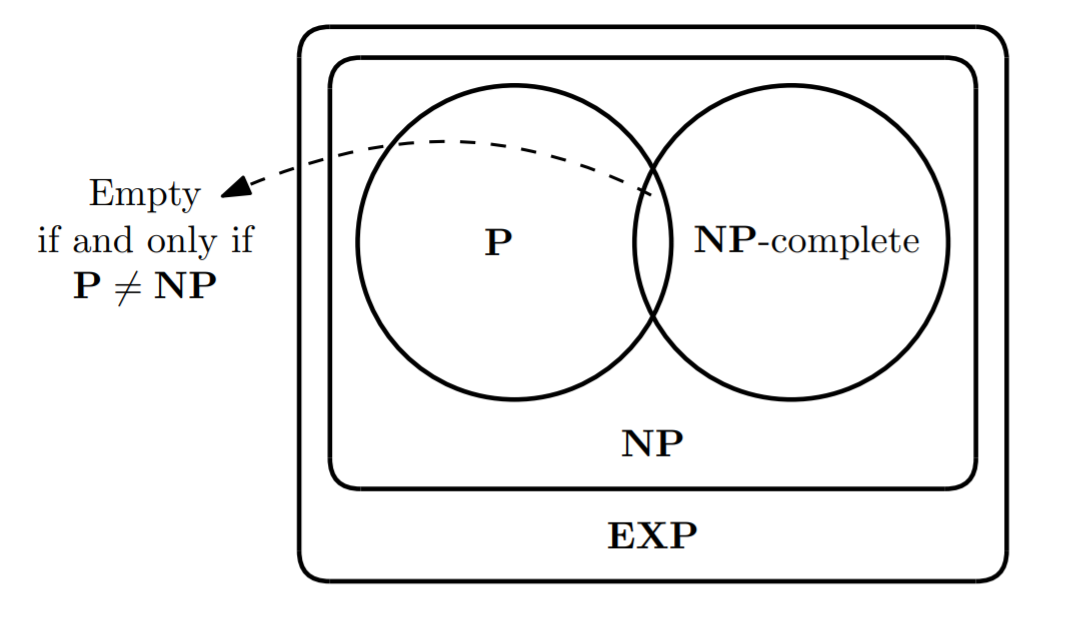
\includegraphics[width = \textwidth]{figures/P-NP-diagram.png}
	\caption{\( \P \subseteq \NP \subseteq \EXP\).
		It is not known whether \NP~and \P~are equal or different, same for \NP~and \EXP. We only know that $\P \neq \EXP$.}
	\label{fig:P-NP-diagram}
\end{marginfigure}


\section{The Cook-Levin Theorem}

\subsection*{Boolean formulas, CNF, and \SAT}

Some of the simplest examples of \NP-complete problems come from propositional logic. A \emph{Boolean formula} over the variables $u_1,\ldots,u_n$ consists of the variables and the logical operators AND ($\wedge$), OR ($\vee$), and NOT ($\neg$). For example, $(u_1 \wedge u_2) \vee (u_2 \wedge u_3) \vee (u_3 \wedge u_1)$ is a Boolean formula. If $\varphi$ is a Boolean formula over variables $u_1,\ldots,u_n$, and $z \in \{0,1\}^n$, then $\varphi(z)$ denotes the value of $\varphi$ when the variables of $\varphi$ are assigned the values $z$ (where we identify 1 with \textsc{True} and 0 with \textsc{False}). \emph{A formula $\varphi$ is satisfiable if there exists some assignment $z$ such that $\varphi(z)$ is \textsc{True}. Otherwise, we say that $\varphi$ is unsatisfiable.}

The above formula $(u_1 \wedge u_2) \vee (u_2 \wedge u_3) \vee (u_3 \wedge u_1)$ is satisfiable, since the assignment $u_1 = 1, u_2 = 0, u_3 = 1$ satisfies it. In general, an assignment $u_1 = z_1, u_2 = z_2, u_3 = z_3$ satisfies the formula iff at least two of the $z_i$'s are 1.

A Boolean formula over variables $u_1,\ldots,u_n$ is in \emph{CNF form} (shorthand for \emph{Conjunctive Normal Form}) if it is an AND of OR's of variables or their negations. For example, the following is a 3CNF formula: (here and elsewhere, $\overline{u_i}$ denotes $\neg u_i$)
\[
	(u_1 \vee \overline{u_2} \vee u_3) \wedge (u_2 \vee \overline{u_3} \vee u_4) \wedge (\overline{u_1} \vee u_3 \vee \overline{u_4})
\]
More generally, a CNF formula has the form
\[
	\bigwedge_i \left(\bigvee_j v_{ij}\right)
\]
where each $v_{ij}$ is either a variable $u_k$ or its negation $\overline{u_k}$. The terms $v_{ij}$ are called the \emph{literals} of the formula and the terms $(\bigvee_j v_{ij})$ are called its \emph{clauses}. A $k$CNF is a CNF formula in which all clauses contain at most $k$ literals. We denote by \SAT the language of all satisfiable CNF formulae and by \kSAT{3} the language of all satisfiable 3CNF formulae.


\begin{theorem}[Cook-Levin]
	The following two languages
	\begin{align*}
		\SAT     & = \{\llcorner F\lrcorner | F \text{ is a satisfiable CNF}\}  \\
		\kSAT{3} & = \{\llcorner F\lrcorner | F \text{ is a satisfiable 3CNF}\}
	\end{align*}
	are \textbf{NP-complete}.
	\label{thm:cook-levin}
\end{theorem}
\begin{proof}[sketch]
	The steps for proving Theorem~\ref{thm:cook-levin} are the following.
	Both \SAT~and \kSAT{3}~are clearly in \NP, since a satisfying assignment can serve as the certificate that a formula is satisfiable. Thus we only need to prove that they are \NP-hard. We do so by (a) proving that \SAT~is \NP-hard and then (b) showing that \SAT is polynomial-time Karp reducible to \kSAT{3}. This implies that \kSAT{3}~is \NP-hard by the transitivity of polynomial-time reductions. See e.g. Section 2.3 of \citet{Arora2009}.
\end{proof}

\section{Proving the hardness of a problem}

The only way to prove that a problem is hard is to prove the language is \NP-complete, in this way we have proven that the problem is not so hard (being in \NP) but not so easy either (unless $\P = \NP$ of course ).

But how can we prove that a language \(\lang{L}\) is \NP-complete?\\

If we want to prove $\lang{L}$ to be \NP-complete, we have to prove two statements:
\begin{enumerate}
	\item That $\lang{L}$ is in \NP.
	      \begin{itemize}[noitemsep,topsep=0pt,parsep=0pt,partopsep=0pt]
		      \item This amounts to showing that there are $p$ polynomial and $\mathcal{M}$ polytime TM such that $\lang{L}$ can be written as
		            $$\lang{L} = \{x \in \{0,1\}^* \mid \exists y \in \{0,1\}^{p(|x|)}.\mathcal{M}(x,y) = 1\}$$
		            which is typically rather easy.
	      \end{itemize}
	\item That any other language $\lang{H} \in$ \NP{} is such that $\lang{H} \leq_p \lang{L}$.
	      \begin{itemize}[noitemsep,topsep=0pt,parsep=0pt,partopsep=0pt]
		      \item We can of course prove the statement directly.
		      \item More often (e.g. when showing 3SAT \NP-complete), one rather proves that $\lang{J} \leq_p \lang{L}$ for a language $\lang{J}$ which is already known to be \NP-complete.
		      \item This is correct, simply because $\leq_p$ is transitive (Theorem~\ref{thm:pre-order-reduc-p=np})
		            \begin{gather*}
			            \vdots \\
			            \lang{H} \xrightarrow{\leq_p} \lang{J} \xrightarrow{\leq_p} \lang{L} \\
			            \vdots
		            \end{gather*}
	      \end{itemize}
\end{enumerate}

\section{Examples of \NP-complete problems}

\subsection{\INDSET}
The \textbf{Independent Set} of a graph $\mathbb{G}$ with vertex set $V$ and edges set $E$ defined as follows
\[
	\INDSET = \{ \langle \mathbb{G}, k \rangle : \exists S \subseteq V \text{ s.t. } |S| \ge k \text{ and } \forall u,v \in S, (u,v) \notin E\} \, .
\]
The Independent Set Problem is the problem of determining whether a graph $\mathbb{G}$ admits an independent set of size at least $k$.

\emph{input}: $(\mathbb{G},k)$\\
\emph{output}: $1$ iff \(\exists S \subseteq V\) s.t. \(|S|\geq k\) \(\land\) \(\forall v,u \in S\) \((v,u) \notin E\)


\subsection{\CLIQUE}
\[
	\CLIQUE = \{ \langle \mathbb{G}, k \rangle : \exists S \subseteq V \text{ s.t. } |S| \ge k \text{ and } \forall u,v \in S, u \neq v \implies (u,v) \in E \}
\]

\emph{input}: $(\mathbb{G},k)$\\
\emph{output}: 1 iff $\mathbb{G}$ contains clique of size $k$\\
A clique is a subset W \(\subseteq\) V of its vertices such that any pair v, w \(\in\) W  of distinct vertices is such that (v, w) \(\in\) E . In other words given an undirected graph a clique is a subset of this graph where all the vertices are connected, effectively yielding a complete subgraph.

\subsection{\kSAT{k}}
input: a formula F\\
output: 1 iff F is a satisfiable kCNF\\

\subsection{Vertex Cover or Node Cover}
\emph{input}: $(\mathbb{G},k)$\\
\emph{output}: 1 iff exists a subset of the vertices \(\exists C \subseteq V\) so that \(|C| \leq b\) and \(\forall (v,u) \in E. v\in C\ or\ u\in C\) \\
It means that a node cover of a graph G is a part of the vertices for which we know that at least one vertices for each node is in the cover.

\subsection{Universal Sink (US)}
For having an universal sink we need to have a \emph{directed} graph $\mathbb{G}=(V,E)$. Since we have a directed graph we do not require $E$ to be symmetric. We can represent graphs using the so-called adjacency matrix. So we can write the graph as the pair $\mathbb{G}=(V,A)$ where $A$ is a \(x \times x\) matrix over \binset. If we put a 1 in the position $i,j$ then we have a edge between the vertex $i$ and $j$.

\emph{input}: $\mathbb{G}$\\
\emph{output}: 1 iff exists a vertex \(v_i\) such that \(\forall j,k \leq n\) with \(j \neq i\) we have \(A_{i,k}=0\) and \(A_{j,i}=1\) .\\
It means that a directed graph has universal sink, (at max 1) if it has a vertex so that all the nodes goes into the vertex and nothing comes out of it.

\subsection{Set Packing (SP)}
\emph{input}: $(S_1,...,S_n,k)$\\
\emph{output}: 1 iff \(\exists  \, (P_1,P_2...,P_k) \in (S_1,...,S_n) \) s.t. \(\forall i,j \ i\neq j\ P_i \cap P_j = \emptyset\)  \\
It means that given a set of sets the problems gives 1 only if exists a subset of size k of this set so that every element (set) is independent from one another.

\subsection{Subgraph Isomorphism (SI)}
Given two undirected graphs \(\mathbb{G}_1 = (V_1,E_1)\) and \(\mathbb{G}_2 = (V_2,E_2)\) we say that:
\begin{enumerate}
	\item \(\mathbb{G}_1\) is a subgraph of \(\mathbb{G}_2\) if and only if \(V_1 \subseteq V_2\) and \(E_1 = E_2 \cap (V_1 \times V_1)\)
	\item A function \(h: V_1 \rightarrow V_2\) is a homomorphism from \(\mathbb{G}_1\) to \(\mathbb{G}_2\) if and only if (v,u)\( \in E_1\) implies \((h(v),h(u)) \in E_2\) .
	\item \(\mathbb{G}_1\) is isomorphic to \(\mathbb{G}_2\) if and only if there exists a bijective (function between the elements of two sets, where each element of one set is paired with exactly one element of the other set, and each element of the other set is paired with exactly one element of the first set.) homomorphism h from \(\mathbb{G}_1\) to \(\mathbb{G}_2\).
\end{enumerate}

\emph{input}: $\mathbb{G}_1 = (V_1,E_1)$ and $\mathbb{G}_2 = (V_2,E_2)$\\
\emph{output}: 1 iff $\mathbb{G}_1$ has a subgraph isomorphic to $\mathbb{G}_2$.

\subsection{SUBSETSUM (SSP)}
In its most general formulation, there is a multiset S of integers and a target-sum T, and the question is to decide whether any subset of the integers sum to precisely T.


\chapter{Elements of Computational Learning Theory}
\label{ch:computational-learning}


\section{Terminology}
\begin{itemize}
	\item \textbf{Instance space} X \(\rightarrow\) is the space from which we take the data. Is the set of instances of objects the learner wants to classify. The data from the instance space are generated through a distribution \textbf{D}, unknown to the learner.
	\item \textbf{Concepts} \(\rightarrow\) it's a collection of objects subsets of the instance space X. This should be thought of as properties of objects.
	\item \textbf{Concepts class} \(\rightarrow\) Collection of concepts
	\item \textbf{Target Concept} \(\rightarrow\) it's the concept the learner wants to build a classifier for
	\item \textbf{Representation class} \(\rightarrow\) we talk about representation class when we have a concept with non constant space to represent it, it requires size(e) bits with \(e \in C\).
\end{itemize}

\section{The General Model}
Every learning algorithm is designed to learn concepts from a concept class C but it does not know the target concept c, nor the associated distribution D.\\
The interface of every learning algorithm can be described in the following way
\begin{figure}[H]
	\centerline{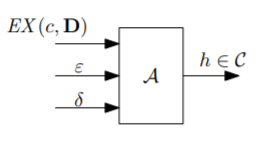
\includegraphics[scale=1]{figures/old/learning}}
\end{figure}
\begin{itemize}
	\item \(\epsilon\) is the \textbf{error parameter}, while \(\delta\) is the \textbf{confidence parameter}.
	\item EX(c,D) is called the \textit{oracle}, a procedure that A can call as many times she wants, and which return an element x from the distribution D, labelled according to whether it is in c or not. Think of it as labeled data.
	\item The error of any \(h \in C\) is defined as \(error_{D,c} = Pr_{x\sim D}[h(x) \ne c(x)]\)
\end{itemize}
So the general model will be:
\begin{figure}[H]
	\centerline{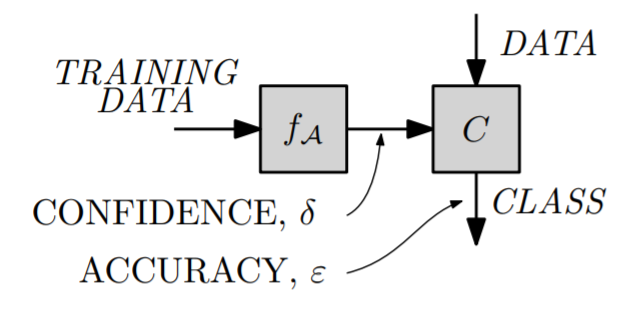
\includegraphics[scale=0.5]{figures/old/learning1}}
\end{figure}
1-\(\delta\) is the probability for which we obtain a classifier with accuracy <\(\epsilon\) .\\
\section{PAC learnable and efficiently PAC learnable}
PAC learnable is the equivalent of a function that can be computed, of a language that can be decided. A concept class is PAC learnable if there is an algorithm that can learn it. If the rime complexity of A is bounded by a polynomial in \(\frac{1}{\epsilon}\) and \(\frac{1}{\delta}\) we say that C is efficiently PAC learnable. The complexity of A is measured taking into account the number of calls to the oracle.

\section{The PAC learning model}

\begin{note}
	A Reference is given by Chapter 2 of \citet{Mohri2018}\sidecite{Mohri2018}

\end{note}

We first introduce several definitions and the notation needed to present the PAC
model.

We denote by $\mathcal{X}$ the set of all possible examples or instances.
$\mathcal{X}$ is also sometimes referred to as the \textbf{input space} or \textbf{instant space}.
The set of all possible \textbf{labels} or target values is denoted by $\mathcal{Y}$.
For the purpose of this introductory treatment, we will limit ourselves to the case where $\mathcal{y}$ is reduced to two labels, $\mathcal{Y} = \binset$, which corresponds to the so-called binary classification.
The results can then be extended to generalized version of $Y$.

A \textbf{concept} $c: \mathcal{X} \to \mathcal{Y}$ is a mapping from $\mathcal{X}$ to $\mathcal{Y}$.
Since $\mathcal{Y} = \binset$, we can identify $c$ with the subset of $\mathcal{X}$ over which it takes the value 1.
Thus, in the following, we equivalently refer to a concept to learn as a mapping from $\mathcal{X}$ to \binset, or as a
subset of $\mathcal{X}$.
As an example, a concept may be the set of points inside a triangle
or the indicator function of these points. In such cases, we will say in short that
the concept to learn is a triangle.

A \textbf{concept class} is a set of concepts we may wish to learn and is denoted by $\mathcal{C}$. This could, for example, be the set of all triangles in the plane.
We assume that examples are independently and identically distributed (i.i.d.)
according to some fixed but unknown distribution $\mathcal{D}$.

The learning problem is then formulated as follows.
The learner considers a fixed set of possible concepts
$\mathcal{H}$, called a \textbf{hypothesis set}, which might not necessarily coincide with $C$.
It receives a sample $S = (x_1,...,x_m)$ drawn i.i.d. according to $\mathcal{D}$ as well as the labels
$(c(x_1),...,c(x_m))$, which are based on a specific target concept $c \in C$ to learn. The
task is then to use the labeled sample $S$ to select a hypothesis $h \in \mathcal{H}$ that has a
small generalization error with respect to the concept $c$. The generalization error
of a hypothesis $h \in \mathcal{H}$, also referred to as the risk or true error (or simply error)
of $h$ is denoted by $R(h)$ and defined as follows.


\begin{definition}[Generalization error]
	Given a hypothesis $h \in \mathcal{H}$, a target concept $c \in \mathcal{C}$, and an underlying distribution $\mathcal{D}$, the generalization error or risk of $h$ is defined by
	\begin{equation}
		R(h) = \mathbb{P}_{x\sim\mathcal{D}}[h(x) \neq c(x)] = \mathbb{E}_{x\sim\mathcal{D}}[1_{h(x)\neq c(x)}],
	\end{equation}
	where $1_\omega$ is the indicator function of the event $\omega$.
\end{definition}

The generalization error of a hypothesis is not directly accessible to the learner
since both the distribution $\mathcal{D}$ and the target concept care unknown. However, the
learner can measure the empirical error of a hypothesis on the labeled sample $S$.

\begin{definition}[Empirical error]
	Given a hypothesis $h \in \mathcal{H}$, a target concept $c \in \mathcal{C}$, and a sample $S = (x_1,\ldots,x_m)$, the empirical error or empirical risk of $h$ is defined by
	\begin{equation}
		\hat{R}_S(h) = \frac{1}{m}\sum_{i=1}^m 1_{h(x_i)\neq c(x_i)}.
	\end{equation}
\end{definition}
Thus, the empirical error of $h \in \mathcal{H}$ is its average error over the sample $S$, while the
generalization error is its expected error based on the distribution $\mathcal{D}$.

\begin{definition}[PAC-learning]
	A concept class $\mathcal{C}$ is said to be PAC-learnable if there exists an algorithm $\mathcal{A}$ and a polynomial function $poly(\cdot,\cdot,\cdot,\cdot)$ such that for any $\epsilon > 0$ and $\delta > 0$, for all distributions $\mathcal{D}$ on $\mathcal{X}$ and for any target concept $c \in \mathcal{C}$, the following holds for any sample size $m \geq poly(1/\epsilon, 1/\delta, n, size(c))$:
	\begin{equation}
		\mathbb{P}_{S\sim\mathcal{D}^m}[R(h_S) \leq \epsilon] \geq 1-\delta.
	\end{equation}
\end{definition}
\section{Exercises 1}

\subsection{Exercise 1}
Write a TM that computes the sum of two binary numbers \(a,b \geq 0\).\\
This exercise is quite complex, let's divide it in different parts. The idea is to increment by 1 the number \(a\) and decrement by 1 the number \(b\) until b is 0.\\
So first we build a TM that increment by 1 a number:
\begin{figure}[H]
	\centerline{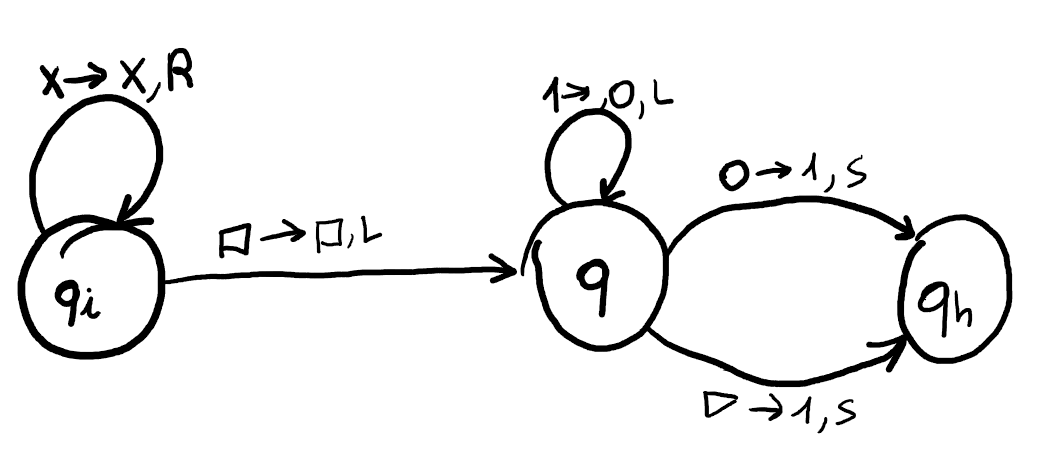
\includegraphics[scale=0.4]{figures/old/TM_increment_1}}
\end{figure}
This will have as alphabet:  \(\Gamma = \{\rhd, 0, 1,  \square\}\) \\
It will have the following states \(\mathcal{Q} = \{q_i, q, q_h\}\) \\
And will have the following transition function:\\
\(\delta (q_i, x) = (q_i, x, R)\)  \\
\(\delta (q_i, \square ) = (q, \square, L)\)  \\
\(\delta (q, 1 ) = (q, 0, L)\) \\
\(\delta (q, 0 ) = (q_h, 1, S)\) \\
\(\delta (q, \rhd ) = (q_h, 1, S)\) \\
Now we need a decrement TM:
\begin{figure}[H]
	\centerline{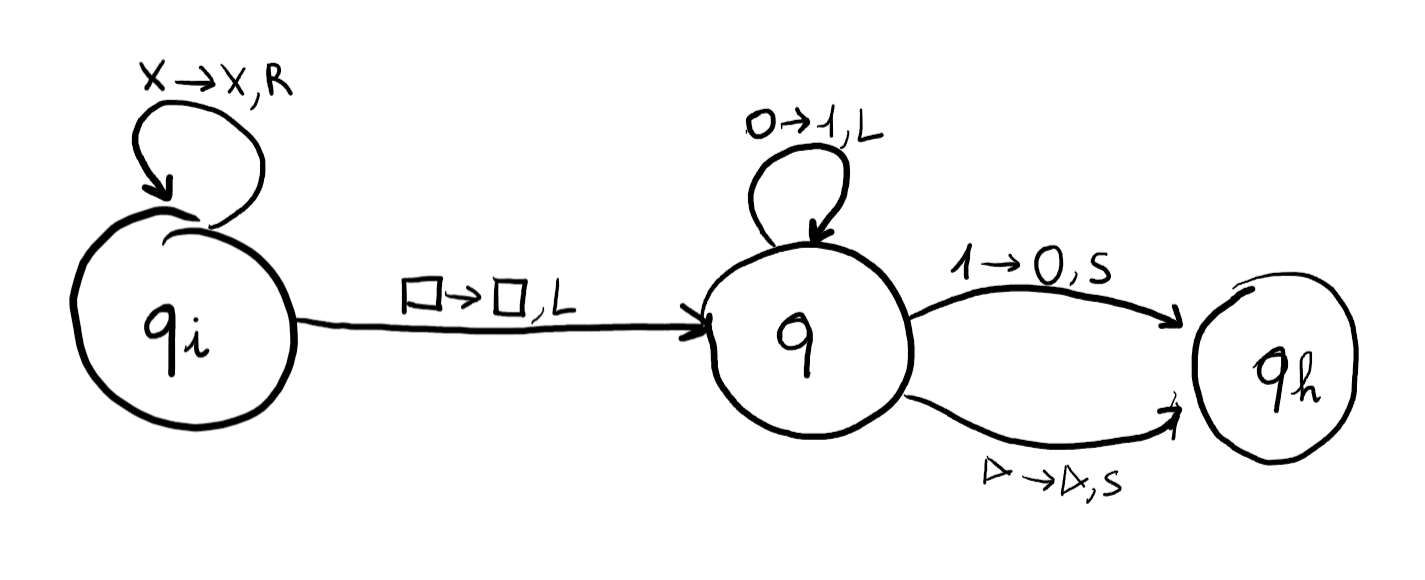
\includegraphics[scale=0.4]{figures/old/TM_decrement_1}}
\end{figure}
This will have as alphabet:  \(\Gamma = \{\rhd, 0, 1,  \square\}\) \\
It will have the following states \(\mathcal{Q} = \{q_i, q, q_h\}\) \\
And will have the following transition function:\\
\(\delta (q_i, x) = (q_i, x, R)\)  \\
\(\delta (q_i, \square ) = (q, \square, L)\)  \\
\(\delta (q, 0 ) = (q, 1, L)\) \\
\(\delta (q, 1 ) = (q_h, 0, S)\) \\
\(\delta (q, \rhd ) = (q_h, \rhd, S)\) \\

So putting all together we will obtain our TM that does the addition of two number. The input will be something like \(...\rhd 010001+0110\square \square...\) .
\begin{figure}[H]
	\centerline{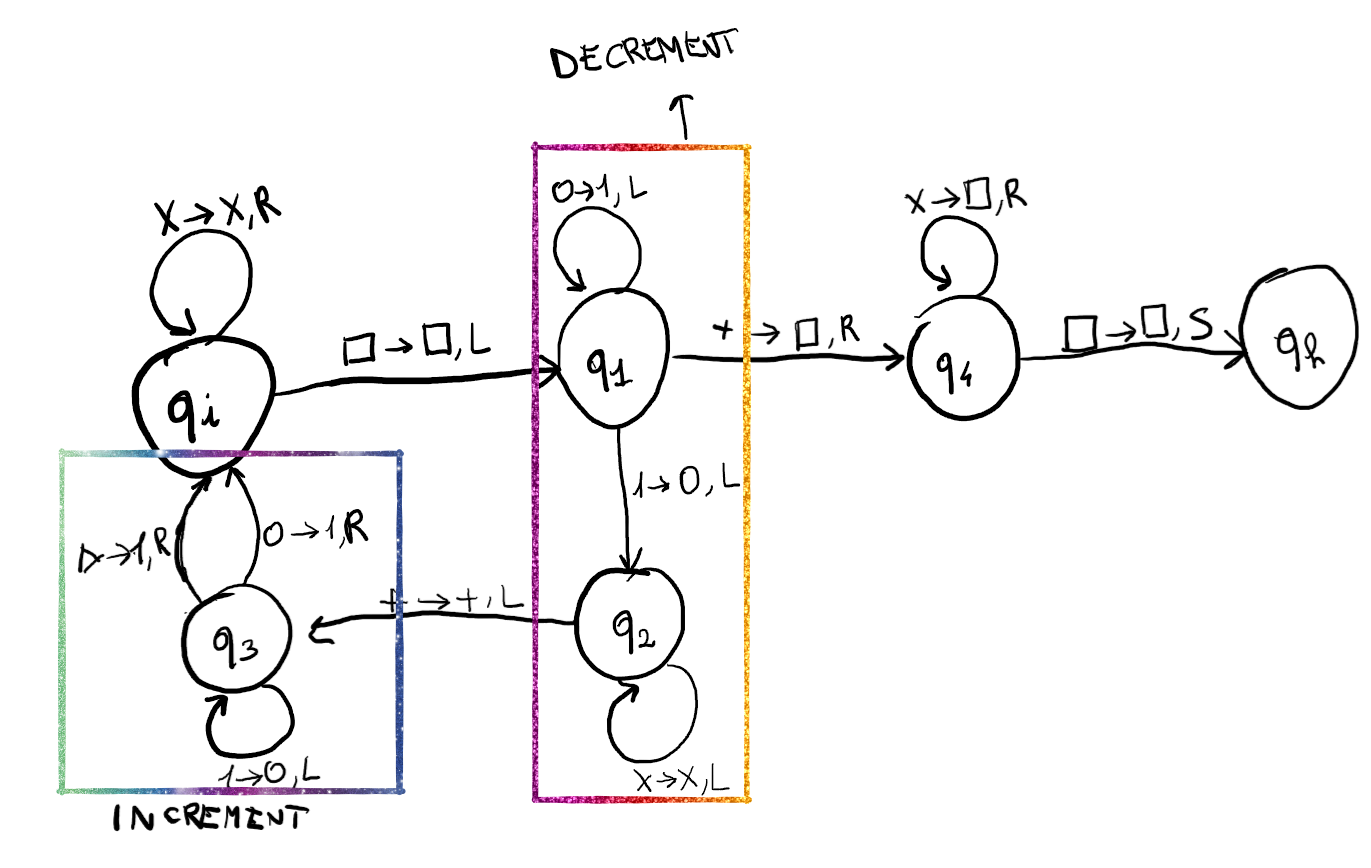
\includegraphics[scale=0.4]{figures/old/TM_addition}}
\end{figure}
This will have as alphabet:  \(\Gamma = \{\rhd, +, 0, 1,  \square\}\) \\
It will have the following states \(\mathcal{Q} = \{q_i, q_1,q_2,q_3,q_4, q_h\}\) \\
And will have the following transition function:\\
\(\delta (q_i, x) = (q_i, x, R)\)  \\
\(\delta (q_i, \square ) = (q, \square, L)\)  \\
... \\

\subsection{Exercise 2}
Write a TM that accept palindromes i.e. write a TM \(\mathcal{M}\) s.t. \(\mathcal{L}(M) = \{w \in \{0,1\}^* | w \text{ is palindrome}\}\) \\
The idea to build this TM is to control if the first and the last digit are equal, if they are equal we substitute them with \(\rhd, \square\) and we continue, if they are different I go into the reject state. If I have an empty string then I can go in the accept state.
\begin{figure}[H]
	\centerline{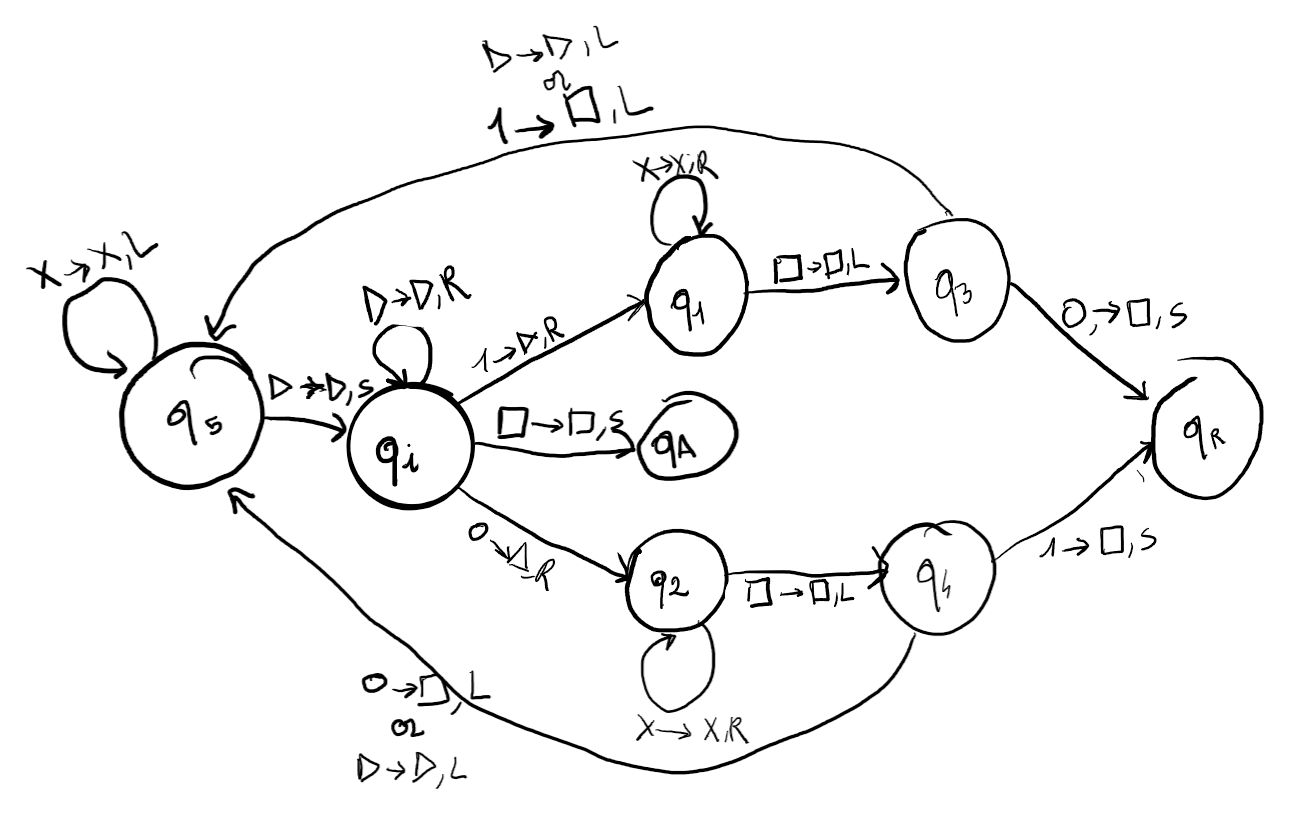
\includegraphics[scale=0.4]{figures/old/TM_palindrome}}
\end{figure}

\subsection{Exercise 3 }
Determine if the following property is \textbf{decidable}:\\
\(P = \{\llcorner N\lrcorner | \mathcal{L}(N) \ infinite \}\) \\
meaning "set of TM so that the languages is infinite.\\
To determine if it is decidable we use the Rice's Theorem. To apply Rice's Theorem we have to prove two things:
\begin{itemize}
	\item P is \textbf{non-trivial}
	\item P is \textbf{extensional}
\end{itemize}
To say that P is \textbf{non-trivial} we have to prove two things:
\begin{itemize}
	\item \(P \neq \emptyset\)
	\item \(\exists N \text{so that }  \llcorner N\lrcorner \notin P\)
\end{itemize}
For the first point we have to prove that exists a TM that accept a language with infinite cardinality:
\begin{figure}[H]
	\centerline{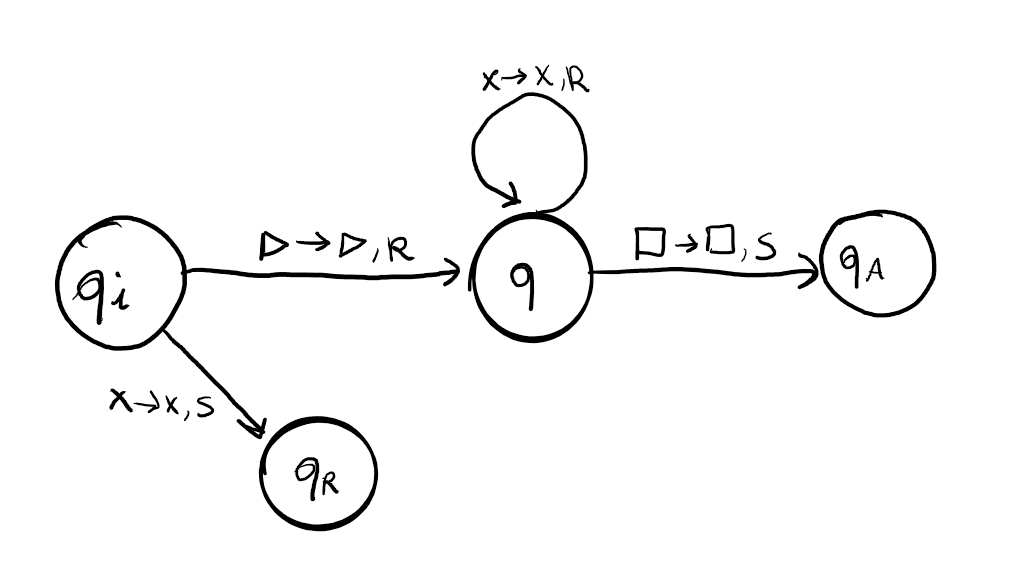
\includegraphics[scale=0.4]{figures/old/TM_always_accept}}
\end{figure}
it never happen that it fails because, the first symbol is always \(\rhd\) .\\
The second thing to prove for P not to be trivial is that exists a TM \(\mathcal{M}\) that does not belong to P:
\begin{figure}[H]
	\centerline{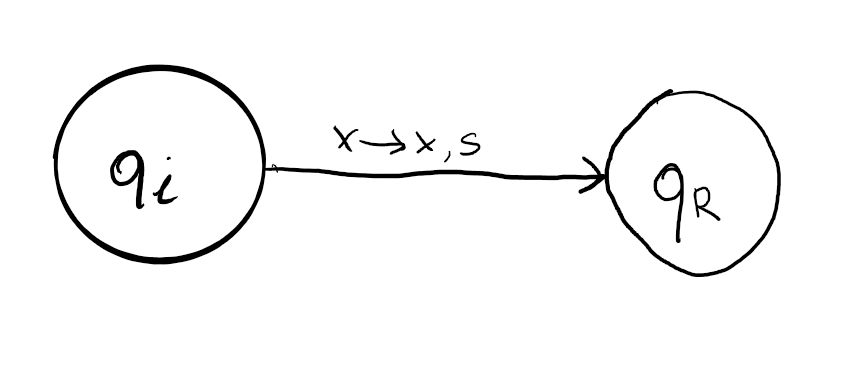
\includegraphics[scale=0.4]{figures/old/TM_always_reject}}
\end{figure}
To say that P is \textbf{extensional} we can say that if we assume that \(\mathcal{L}(M) = \mathcal{L}(N)\) and \(\llcorner M\lrcorner \in P\) we have to show that also \(\llcorner N \lrcorner \in P\). We start by saying that because \(\llcorner M\lrcorner \in P\) iff \(|\mathcal{L}(M)|=\infty\) and we know that   \(\mathcal{L}(M) = \mathcal{L}(N)\), then \(|\mathcal{L}(N)|=\infty\), hence \(\llcorner N \lrcorner \in P\).\\
So from this we can conclude that P is \textbf{undecidable}.

\subsection{Exercise 4 (Construct a TM that decides a language)}
\begin{lstlisting}[breaklines]
Construct a deterministic TM of the kind you prefer, which decides the following language:
L = {w in {0,1}* | between any pair of occurrences of 0 in w there are an odd number of 1s}
Study the complexity of TM you have defined.

solution:
the alphabet is {0,1, start, blank}
the states are {qinit, q1,q2,q3,q4,qa,qr}
the transition function is :
delta (qinit, start) = (q1,start,R)
delta (q1,1)= (q1,1,R)
delta (q1,0)= (q2,0,R)
delta(q1,blank)= (qa, blank, S)
delta(q2, 1)=(q3,1,R)
delta(q2,0)=(q3,0,S)
delta(q2,blank)=(qa, blank,S)
delta(q3, 1)= (q4,1,S)
delta(q3, blank)=(qa, blank,S)
delta(q3,0)= (q2,0,R)
delta(q4, 1)= (q3,1,S)
delta(q4,0)= (qr,0,S)
delta(q4,blank)= (qa, blank, S)

The TM has to go through the tape only one time, so the complexity is linear O(n).
\end{lstlisting}
\begin{figure}[H]
	\centerline{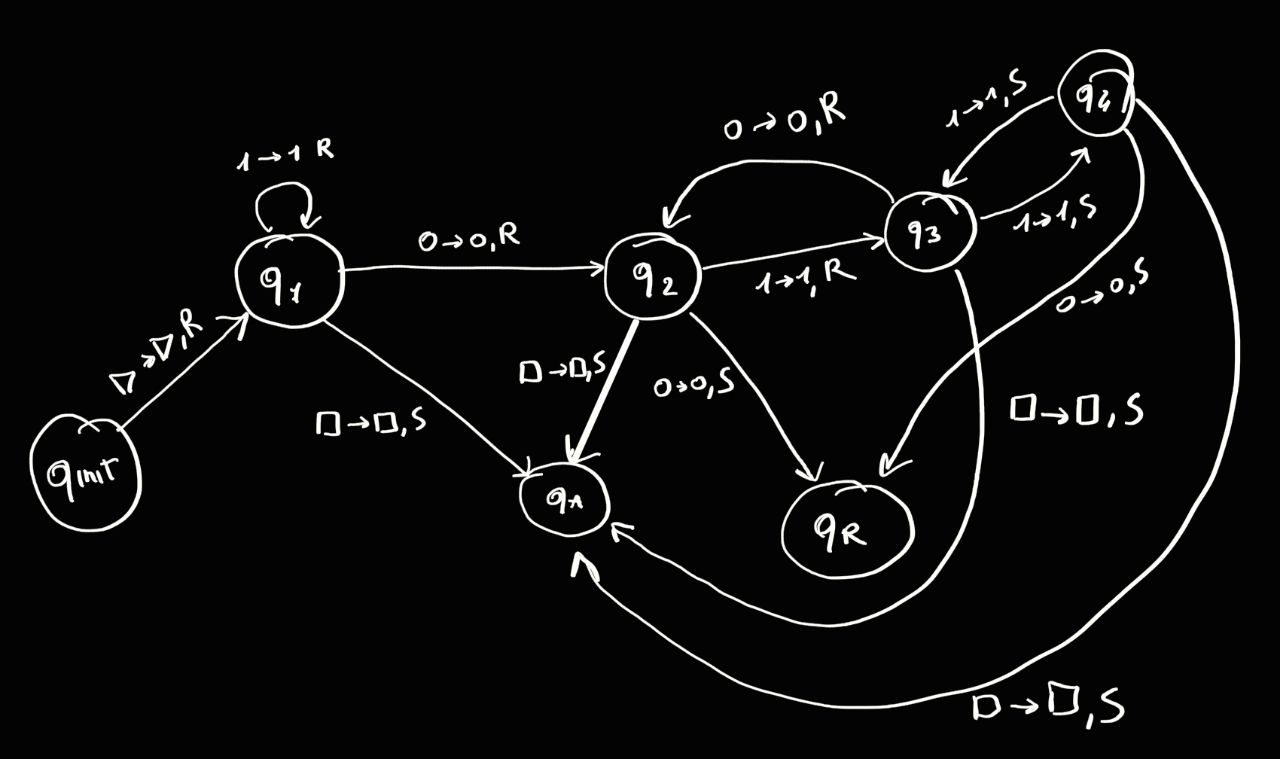
\includegraphics[scale=0.2]{figures/old/TM_1_odd}}
\end{figure}

\subsection{Exercise 5 (Construct a TM that decides a language)}
\begin{lstlisting}[breaklines]
Construct a deterministic TM of the kind you prefer, which decides the following language:
L = {w in {0,1}* | every 1 occurring in w is immediately followed by a 0}
Study the complexity of TM you have defined.
solution 
alphabet: {0,1,start, blank}
states: {qinit, q1,q2,qa,qr}
transition functions:
delta(qinit, start)= (q1,start, R)
delta(q1,0)= (q1,0,R)
delta(q1,1)=(q2,1,R)
delta(q1, blank)=(qa, blank, S)
delta(q2, 0)=(q1,0,R)
delta(q2,1)=(qr,1,S)
delta(q2, blank)=(qr, blank, S)

The complexity of the TM is linear  because it goes through the tape only one time one bit at a time.
\end{lstlisting}
\begin{figure}[H]
	\centerline{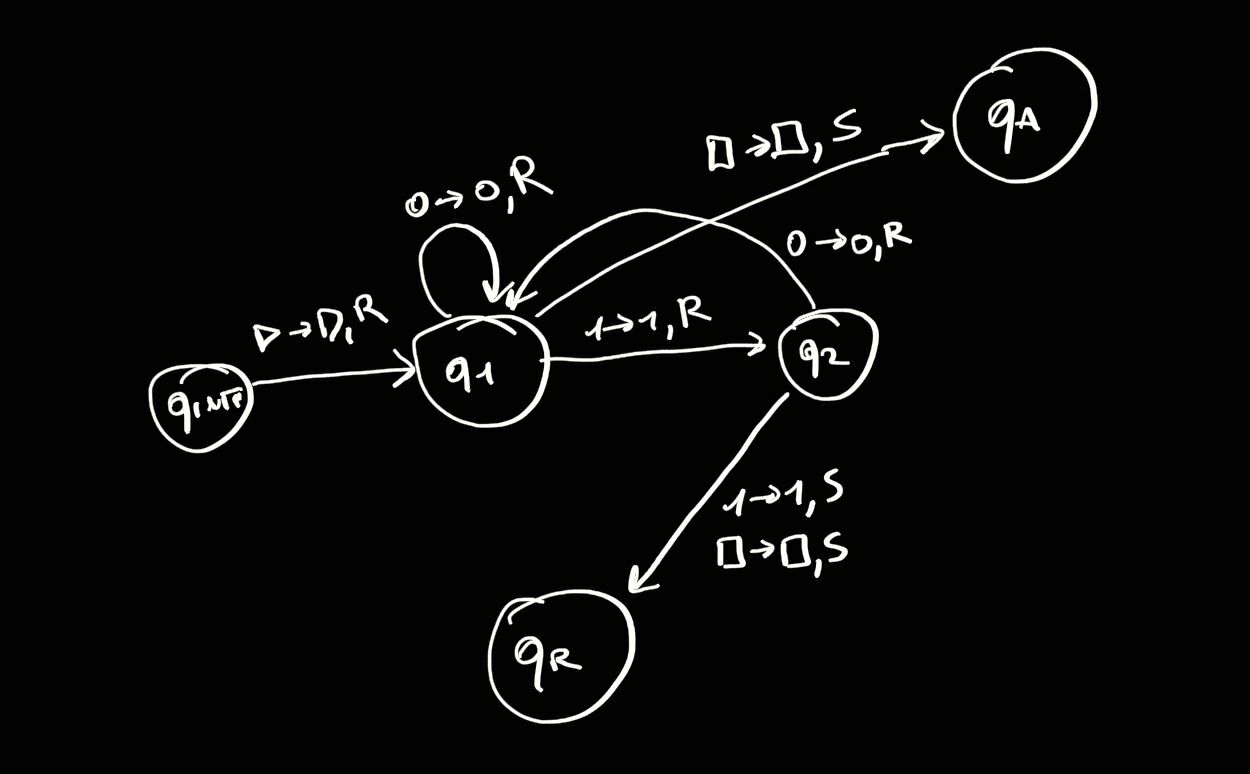
\includegraphics[scale=0.2]{figures/old/TM_2}}
\end{figure}
\subsection{Exercise 6 (Construct a TM that decides a language)}

\begin{lstlisting}[breaklines]
Construct a deterministic TM of the kind you prefer, which decides the following language:
L = {w in {0,1}* | does not contains 10 as substring}
study the complexity of the TM you have defined.

solution:
alphabet: {0,1,start, blank}
states: {qinit, q1,q2,qa,qr}
transition function :
delta(qinit, start)= (q1, start, R)
delta(q1,0)= (q1, 0,R)
delta(q1, 1)=(q2,1,R)
delta(q1, blank)=(qa, blank,S)
delta(q2,0)=(qr,0,R)
delta(q2,1)=(q2,1,R)
delta(q2, blank)=(qa, blank,S)

This TM decides the language in polynomial time, in fact it goes through the tape only one time, one symbol at a time. In particular it is linear, DTIME(n) where n is the size of the input string.
\end{lstlisting}

\section{Exercises 2}

\subsection{Exercise 1}
\textbf{Prove that a problem is in P}\\
Given a list \(A = [a_1,...,a_n]\) s.t. \(\forall i \  a_i \in N \) return an index \(i \in \{1,...,n\}\) s.t. \(A[i] = v\), where \(v \in N\), if any, otherwise return -1. \\
So here we have as input a list A and a natural number v. The result will be a natural number. \\
\textbf{Solution}\\
1. \textbf{Give a pseudo-code}:
\begin{minted}[style=fruity, bgcolor=black]{python}
i <- 1 
while i < n do {
if A[i] == v return i
else i <- i +1
}
return -1

\end{minted}
2. \textbf{encode the input of the program as bit string}, and show that it can be done in polynomial time:\\
We know that if I want to encode a natural number n I will need a number of bit that is \(log(n)+1\). One possible way to encode a list of natural number is to separate them by a symbol ($\#$) so that now our alphabet will have 3 symbols (0, $\#$,1) that will be encoded in binary as (00,01,11). So now to encode a natural number we will need \(2 \cdot (log(n) +1)\) bit, so the total length of the encoding of the input will be :
\[l = |\llcorner (A,v)\lrcorner| = (\sum_{i=1}^n 2 \cdot (log(a_i) +1)) + 2n+ 2(log(v) +1\]
3. \textbf{Prove that the number of basic instructions of our pseudo-code is bounded by a polynomial in l}\\
In our pseudo-code we have :
\begin{itemize}
	\item 1 assignmente
	\item n iteration (in the worst case)
	      \begin{itemize}
		      \item 1 inequality check
		      \item a conditional branching
		      \item 1 equality check
		      \item 1 addition
		      \item 1 assignment
	      \end{itemize}
	\item a return instruction
\end{itemize}
So I have n iteration in which we do c number of instruction and out of the iteration we have b number of instruction so the total number of instruction is: \(b+n\cdot c \leq p(l)\), meaning that can be bounded by a polynomial in l.\\
4.\textbf{All intermediate results are polynomially bounded in length}\\
i start by 1 and we add 1 for n times so i is polynomially bounded.\\
5. \textbf{Argue that each instruction can be simulated by a turing machine that runs in polytime with respect to l}\\
All the operation done in our code can be simulated by a TM that runs in polytime
\begin{itemize}
	\item assignment
	\item inequelity check
	\item equality check
	\item adding 1
\end{itemize}

\subsection{Exercise 2 (Prove a function to be in FP)}
\begin{lstlisting}[breaklines]
You are required to prove that the following function f in in FP. To do that, you can give a TMs or define some pseudocode. The function is one that, given two strings v,w checks wheter v is a substring of w, namely wheter w contains an exact occurrence of v.

solution:
1. pseudo-code:
n = size(w);
m=size(v);
k=0
 for i in 0..n-1
  if (v[k]==w[i]){
    k++
   }
   else {
   k=0
   }
   return k==m
   
   
2. encode the input as a bit string:
   given n the number of different symbols in the string v and w, we need (log n +1) bit for every symbol, we also need a separation symbol # between characters and a separation symbol between the two string @, so the alphabet {0,1,#,@} will be encoded as {00,01,11, 10} so we need, given k=size(v)+size(w) we have the total size of the encoded input will be:
   size(input) = 2k(log n +1)+ 2k + 2 that is polynomial.

3. number of basic instruction:
-assignment
-assignment
-assignment
-loop 
 -equality check
  -add 1 and assignment
 -assignment
-equality check
so the number of instruction will be a+bn= O(n), where n<size(input) so the number of basic instruction is polynomial with respect to the seize of the input.

4. All intermediate result are bounded polynomially in length:
 k goes from 0 to the size of v and i goes from 0 to the size of w.
 
 5. argue that every instruction can be simulated by a TM that runs in polyomial time:
 We have only assignment, addition of 1 that can be done in polytime by a TM and equality check that can be done in polytime.
\end{lstlisting}

\subsection{Exercise 3 (prove a function to be in FP)}
\begin{lstlisting}[breaklines]
You are required to prove that the following function f is in FP. To do that you can give a TMs or define some pseudocode. The function is one that, given a list L=L1,...,Ln, returns its inverse namely Ln,Ln-1,...,L1.
solution:
1. Pseudocode:
k = size(L)
j = 0 
for i in k-1 to 0
 Inv_L [j] = L[i]
 j++
return Inv_L

2. encoding of the input:
The input is a list so the encoding will be the encoding of each element separated by a symbol  #. We do not know what L1,...,Ln but let's say that they are natural number in this case the encoding would be L1#L2#...#Ln, the alphabet would be {0,1,#}, in bit would be {00,01,11}, so the total length would be 2n(log L +1)+ 2n.
3. number of basic instruction:
The number of basic instruction will be c+ n*a so O(n), where n is the size of the input.
4. each instruction can be simulated by a TM: We can simulate each instruction by a TM, we have assignment, addition of 1 and equality check that can be done in polynomial time by a TM.
5. All data used is polynomial in the input: 
  -k is the size of the input
  -j start from 0 and add 1 for k time, so it will have value k
  -Inv_L has the same size as the input
\end{lstlisting}

\subsection{Exercise 4 (prove a function to be in FP)}
\begin{lstlisting}[breaklines]
You are required to prove that the following function f is in FP. To do that, you can give a TMs or define some pseudocode. The function is one that, given two lists L=L1,...,Ln and P = P1,...,Pn of rational numbers returns their scalar products.

solution:
1. pseudocode
n=size(P)
dot = 0
for i in 0..m
dot = dot + L[i]*P[i]
return dot

2. encode the input 
The input is formed by two list of rational numbers. we need a symbol to separate the two list @, we need a symbol to separate the rational numbers #, a symbol to separate the numerator from the denominator / and and two symbols for the sign so that in total we would have the following alphabet {+,-,0,1,#,@} so we would need 3 bit. we encode the rational number as Sign num/den, where num and den are natural numbers, and so they would need log k +1 bit. In total we would have : 3*2*2*n(log n+1)+ 3*2*n+ 3 that is polynomial.
3. number of basic instruction is polynomial
the number of basic instruction is c+n that is polynomial in the input encoding length
4. each instruction can be simulated by a TM working in poly time: as basic instruction we have assignment, sum, multiplication that could be done in polynomial time.
5. all data used is polynomial in the size of the input:
dot is a natural number, its size is polynomially bounded by the size of the input.
\end{lstlisting}



\section{Exercises 3}
\subsection{Exercise 1}
Suppose clique is the following set: \[\text{CLIQUE} = \{(\mathcal{G}, k) \ | \ \text{ is an undirected graph containing a glique of size at least k }\}\]\\
\textbf{Prove that clique is NP-complete} by showing that \(3SAT \leq_p \text{CLIQUE}\)\\
\textit{Hint: consider any 3CNF F as a graph whose vertices are the occurrences of literals in F}
\\
\textbf{Solution}
A clique is a subset \(W \leq V\) of its vertices such that any pair \(v,w \in W\) of distinct vertices is such that \(\{v,w\} \in E\) . In other words given an undirected graph a clique is a subset of this graph where all the vertices are connected.
\begin{figure}[H]
	\centerline{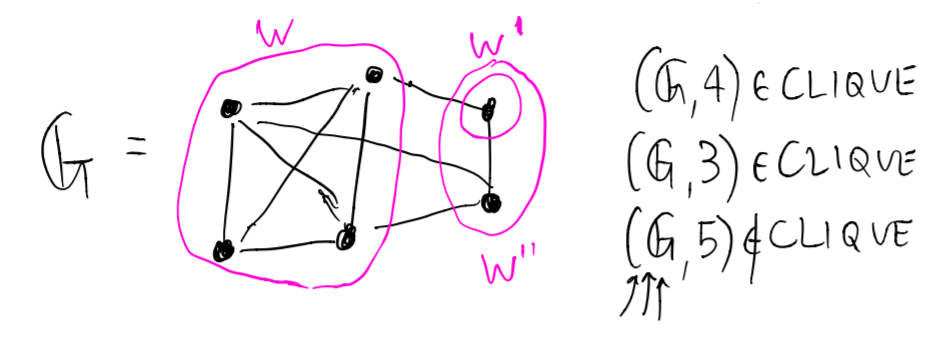
\includegraphics[scale=0.4]{images/clique}}
\end{figure}
So \((\mathcal{G},4)\) belong to clique because in w (pink) I can see that I have at least 4 vertices which are all connected.  \((\mathcal{G},5)\) does not belong to clique because I can't find a subset of the graph where 5 vertices are all connected.\\
The fact that clique in in NP is easy to prove: the certificate, as expected, is a subset \(W \subseteq V\) such that \(W\) has a k-CLIQUE. Indeed:
\begin{itemize}
	\item Its size (which is its cardinality) is smaller than the one of \(\mathcal{G}\).
	\item checking that \(W\) is indeed a clieque of size \(\geq\) to k can be done in quadratic time: it sufficies to check that any pair of distinct vertices \(v,w \in W\) are connected by an edge.
\end{itemize}
About completeness, we want a reduction \(f\) such that for every 3CNF F, \(f(F)\) is a pair \((\mathcal{G}, k)\), and moreover \((\mathcal{G}, k) \in \text{CLIQUE}\) IFF F is satisfiable. So first of all we can observe that a natural way of turning CNFs into graphs consist in introducing a node for each literal in the CNF. So let's see what it means graphically
\begin{figure}[H]
	\centerline{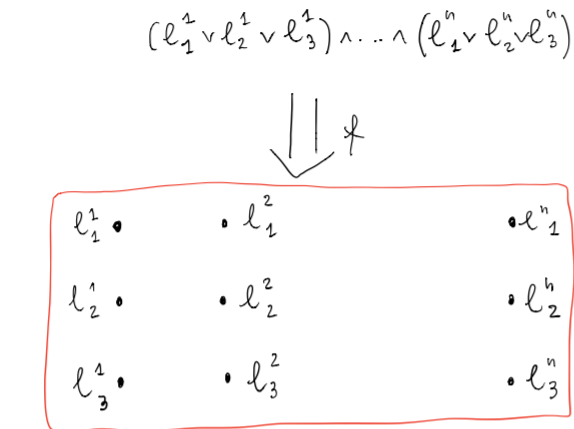
\includegraphics[scale=0.4]{images/clique_1}}
\end{figure}
for every \(i \ne j\) and for every \(s,q \ in \{1,2,3\}\) we have an edge beween \(l_s^i\) and \(l_q^j\) iff the two literals are compatible from a logical point of view, namely iff they don't talk about the same variable in inconsistent ways (for example, we do not have an edge between \(x\) and \(\lnot x\) . \\
The only missing ingredient in the proof is to prove that F is satisfiable IFF \(f(F)\) has a CLIQUE of size equal to the number of clauses in F:
\begin{itemize}
	\item Suppose that F is satisfiable, then there is an assignment of truth value to the variables in F which makes the n clauses of F all \textbf{true}. This means that for every \(i \in \{1,...,n\}\) (the clause) there exists \(s \in \{1,2,3\}\) (the literals inside each clause) such that \(l_s^i\) is true in the assignment. All this literals then are pairwise consistent (i.e. it can't be that \(l_s^i=x \text{ and } l_q^j =\lnot x\) ), the nodes corresponding to these literals in \(f(F)\) are all linked by an edge. Hence \(f(F)\) is indeed a graph which has a clique of size n.
	\item Suppose that the graph \(f(F)\) has a clique of size n. It means that all columns of \(f(F)\) are "involved" in the clique (because there are no edges between nodes in the same column). There is thus a way of choosing for each clause in F one of its literals in such a way as to preserve logical consistency, and this, by definition of logical consistency, means that there is an assignment which makes all these literals true, since we have at least one literal for each clause. The formula F is satisfiable.
\end{itemize}

\subsection{Exercise 2 (prove a language to be in NP)}
\begin{lstlisting}[breaklines]
You are required to prove that the following problem L in in NP. To do that, you can give a TM or define some pseudocode. The language L includes precisely those binary strings which are encodings of pairs in the form (G,t) where G is a graph and t is a natural number, such that the nodes of G can be partitioned into at most t sets in such a way that nodes which are part of distinct sets are not linked by any edge.
 or equivalently:
 You are required to prove that the following problem L in in NP. To do that, you can give a TM or define some pseudocode. The language L includes precisely those binary strings which are encodings of pairs in the form (G,k) where G is a graph and k is a natural number, such that the nodes of G can be assigned a natural number between 1 and k in such a way that nodes which are linked by an edge are assigned distinct natural numbers.
 
Solution:
L = {(G,k) | exists N, if (u,v) belong E, N[u]!=N[v] }
where G = (V,E)
-CERTIFICATE: We take as a certificate N, list of natural number assigned to each node of G.
-CERTIFICATE SIZE: N is a list of size |V| of natural number <k. So the certificate size is O(|V| * log(k) ) , which is polynomial in the size of the input.
-TM FOR CHECKING THE CERTIFICATE (VERIFIER): The TM will have to check if every pair in E has different values in N. So:
	for (u,v) in E
    	if (N[u]==N[v])
         return false
    return true
    
    this has a complexity O(|E|)=O(|V|^2) which is polynomial.
    
    So L is in NP.
   
\end{lstlisting}
\subsection{Exercise 3 (1SAT)}
\begin{lstlisting}[breaklines]
Consider the following problem:
1SAT = {A|A is a satisfiable 1CNF}
To which complexity class does 1SAT belong? Prove your claim.

Solution:
1SAT belong to the complexity class P.
prove:
1. Pseudocode:
n = size(A)[0]
for i in 0..n
 for j in 0..n
   if (A[i][0]==A[j][0] and A[i][1]!=A[j][1])
    return false
return true
2. Encoding of the input:
the input can be encoded as a list of literals, that can be negated or not. We will need a symbol to separate the literals, one to negate a literal so in the end we will have the following alphabet {0,1,#,@} that encoded will be {00,01,10,11}. If k is the number of different literal and n the total number of literals and w is the total number of negated literal w<n, we will have that the total length of the input encoding will be l= 2 (n(log k +1)+ n+ w) that is polynomial in the length of the input.
3. number of basic instruction:
The number of basic instruction is c+b*n^2 which is polynomially bounded with respect to the length of the encoding of the input.
4. basic instruction polynomially bounded with respect to the length of the input encoding:
every instruction can be modeled by a TM that works in polynomial time, equality check, infact, can be done in polynomial time by a TM.
5. Every partial result is polynomially bounded by the length of the input encoding:
i is a natural number that goes from 0 to the size of the input, so it is polynomially bounded.

Follow that 1SAT is in P.
\end{lstlisting}
\subsection{Exercise 4 (ONEINDSET)}
\begin{lstlisting}[breaklines]
We studied the problem INDSET. You are required to classify the subset ONEINDSET of INDSET whose elements are pairs G,k, such that G is an undirected graph such that every node is contained in at most one edge, and k is a natural number. To which complexity class does ONEINDSET belong?

solution:
definition of ONEINDSET 
Input: (G,k)
Output: 1 iff exists I subset V s.t. |I| >=k and for u,v in I then (u,v) not belong to E and for every u s.t exists u,v in E then not exists u,w in E, v!=w.

I can try to prove that ONEINDSET is in P:
Theorem: Let G=(V,E) be an undirected graph. If every v in V is contained in at most one edge then G has an independent set of size |I|=|V|-|E| .
 prove: if I have that every v in V is contained in at most one edge then if I have a pair (u,v) in E then they will not be in any other pair. So I Will have two independent set of size |V|-1, if I apply this for every pair in E, I will have an independent set of size |V|-|E|.
 This theorem allow us to build a simple TM deciding ONEINDSET that trivially works in polynomial time, therefore ONEINDSET is in P.
\end{lstlisting}

\subsection{Exercise 5 (THREECLIQUE)}
\begin{lstlisting}[breaklines]
We studied the problem CLIQUE. You are required to classify the subset THREECLIQUE of CLIQUE consisting of all the pairs (G,3). To which class does THREECLIQUE belong?

solution:
THREECLIQUE belong to the class P.
1. Pseudocode
for i in V
 for j in V
  for k in V
   if (i,j) in E and (i,k) in E and (j,k) in E
    return true
  return false
2. encoding the input
The input is G=(V,E). V can be encoded as a natural number, while E as pairs of natural numbers. We need a symbol # to separate the different natural numbers so our alphabet will be {0,1,#} that encoded will be {00,01,11}. The total bits that we need will be:
l= 2(2*|E|(log(n)+1) + 2|E| + (log V +1) +1)= O(|E|)= O(|V|^2)
3. number of basic instruction:
we have three innested loop from 1 to V, so the total number of instruction is c+b|V|^3= O(|V|^3) which is polynomial in the length of the encoding of the input.
4. basic instruction TM polynomially bounded
The only non-trivial instruction is checking if a pair is connected by an arc, which can be done in O(|E|)=O(|V|^2) = O(l) which is polynomial with respect to the size of the encoding of the input.
5. partial data polynomially bounded 
i,j,k are natural number, their maximum size will be (log |V| +1) bit which is polynomially bounded with respect to the size of the encoding of the input.
\end{lstlisting}
\subsection{Exercise 6 (4SAT)}
\begin{lstlisting}[breaklines]
4SAT = {A | A is a satisfiable 4CNF}
to which complexity class does 4SAT belong? Prove your claim.

solution:
4SAT is NP-Complete.
 -4SAT is in NP
 4SAT = {A | exist P such that A(P)=true}
 P is the certificate and it is an assignment for every variable so its length it's polynomial with respect to the length of A. 
 The TM that has to verify, has to substitute the values of thruthness in A, and this can be done in polynomial time. 
 So 4SAT is in NP.
 -I can reduce 4SAT from 3SAT -> 3SAT <=_p 4SAT
 definition:
  3SAT:
   input: A
   output 1 iff A is satisfiable and 3CNF
 
 4SAT:
  input:A
  output 1 iff A is satisfiable and 4CNF
  
  3SAT <=_p 4SAT means that A in 3SAT iff M(A) in 4SAT  
For each clause of the type (A or B or C) I create two claused of the type (A or B or C or D) and (A or B or C or notD), this way the truth value of D becomes irrelevant to the satisfiability of the 4CNF. The reduction is polytime because I just add a new variable for each clause.
  - for the statement 3SAT =>4SAT, since we created a new variable that for construction is irrelevant, then if a (A or B or C) is true then also (A or B or C or D) and (A or B or C or notD) is true.
  -for the statement 4SAT =>3SAT if I have that (A or B or C or D) and (A or B or C or notD) is satisfiable, since we have bot D and notD in different clauses it is irrelevant. So without D the formula will be satisfiable in 3SAT.
\end{lstlisting}

\subsection{Exercise 7 (2SAT)}
\begin{lstlisting}[breaklines]
Consider the following problem:
2SAT = {A|A is a satisfiable 2CNF}
To which complexity class does 2SAT belong? Prove your claim.

Solution:
This is a quite complex problem to solve, but it has been solve and 2SAT belong to P. The dimonstration is based on the fact that I can rewrite (A or B) as ((notA => B) and (notB => A))
\end{lstlisting}

\subsection{Exercise 8 ( NODECOVER reduction)}
\begin{figure}[H]
	\centerline{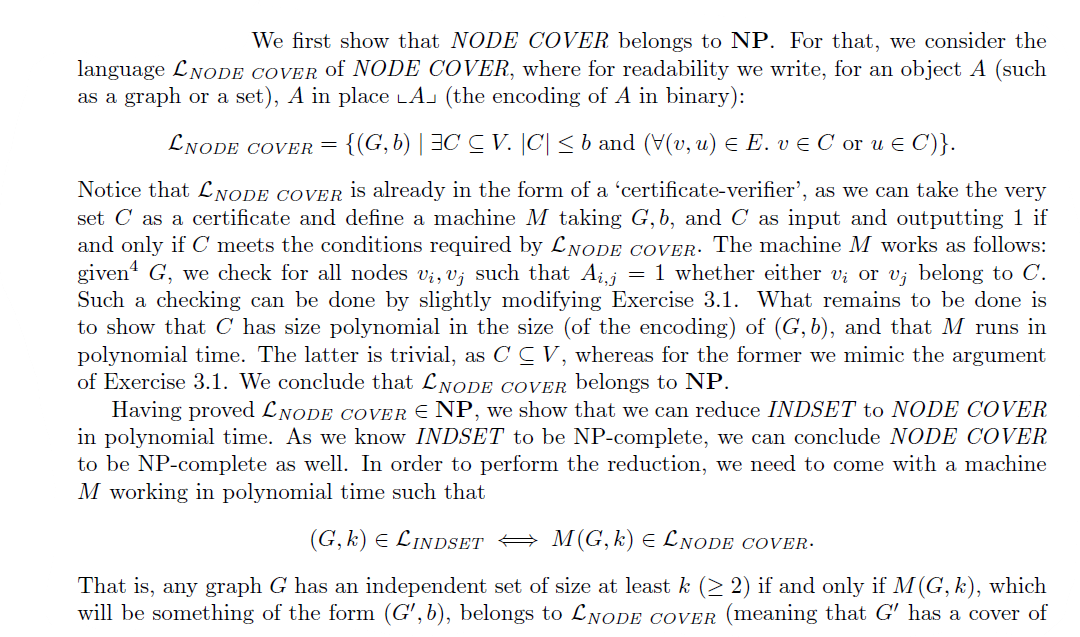
\includegraphics[scale=0.8]{images/Nodecover1}}
\end{figure}
\begin{figure}[H]
	\centerline{
\includegraphics[scale=0.8]{images/Nodecover2}}
\end{figure}
\subsection{Exercise 9 ( SET PACKING reduction)}
\begin{figure}[H]
	\centerline{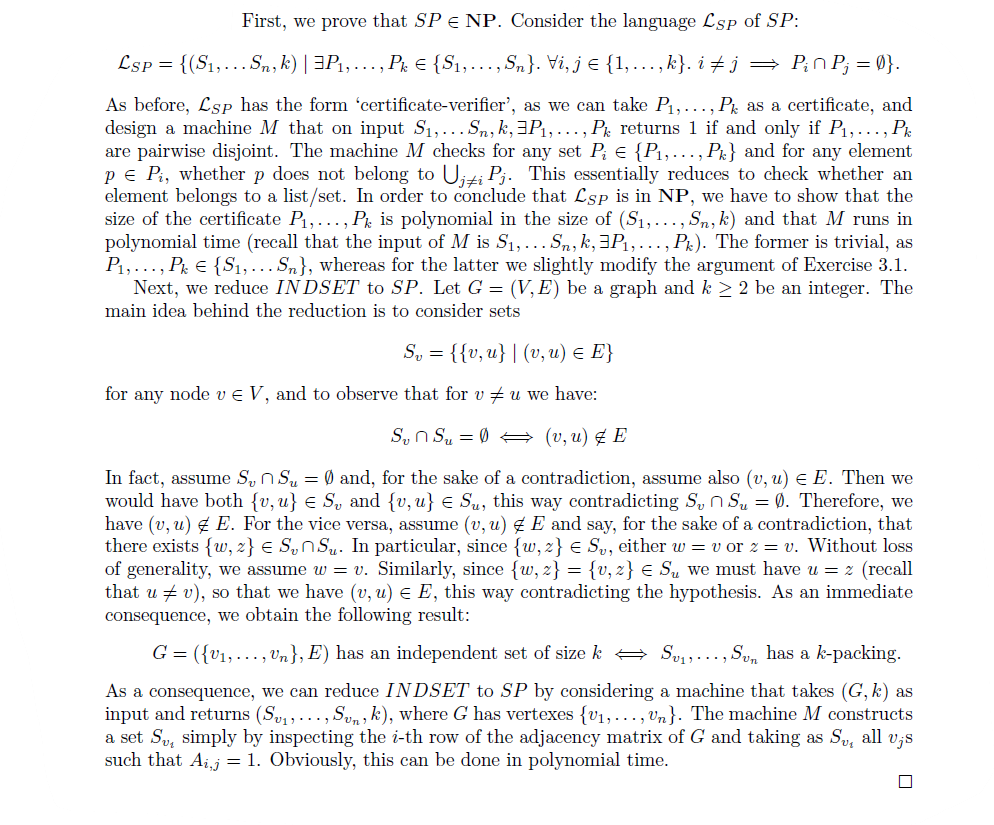
\includegraphics[scale=0.8]{images/SP}}
\end{figure}

% \section{Theory exercises (with solutions)}
%  \begin{figure}[H]
% \centerline{
\includegraphics[scale=0.5]{figures/old/theory/1}}
% \end{figure}
%  \begin{figure}[H]
% \centerline{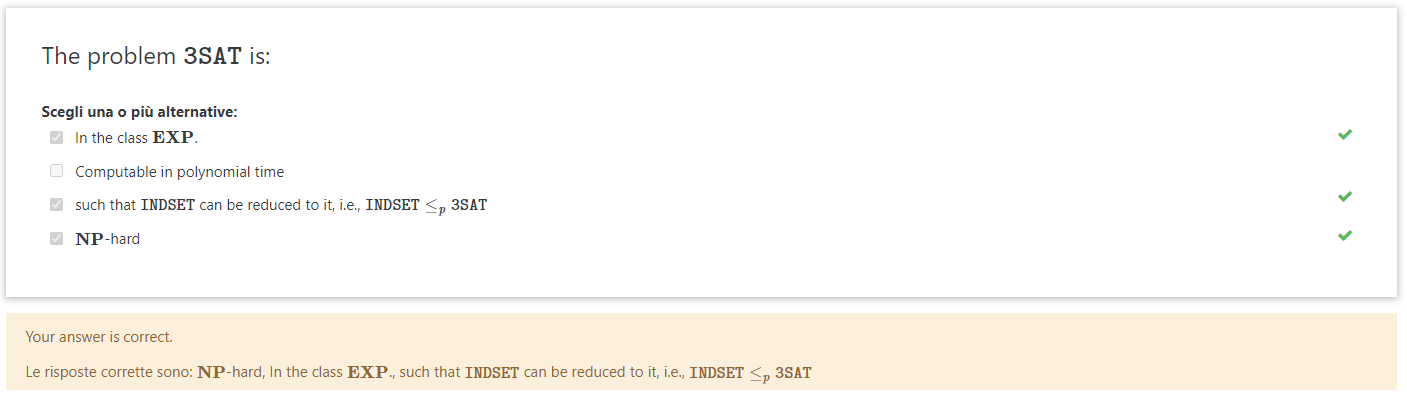
\includegraphics[scale=0.5]{figures/old/theory/2}}
% \end{figure}
%  \begin{figure}[H]
% \centerline{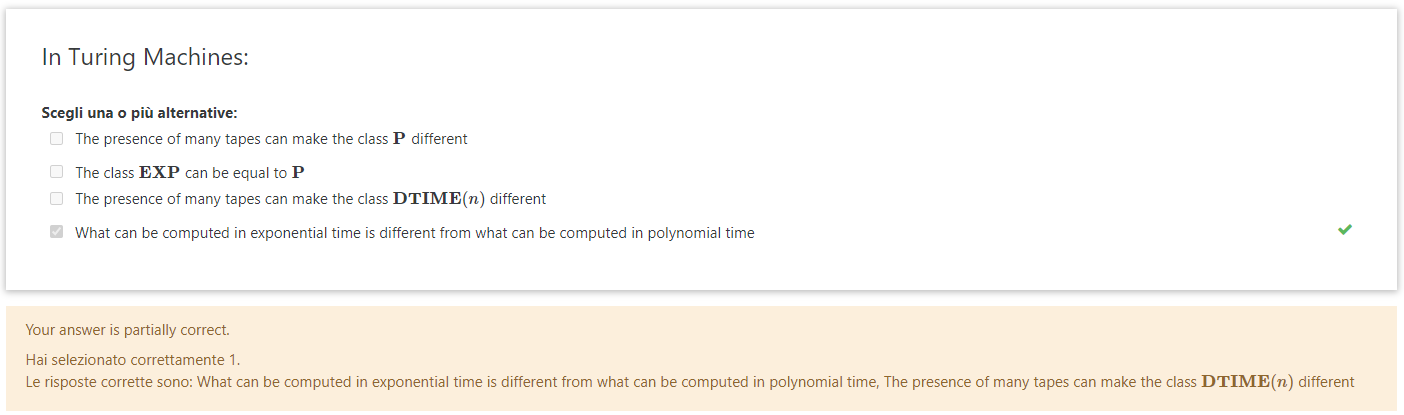
\includegraphics[scale=0.5]{figures/old/theory/3}}
% \end{figure}
%  \begin{figure}[H]
% \centerline{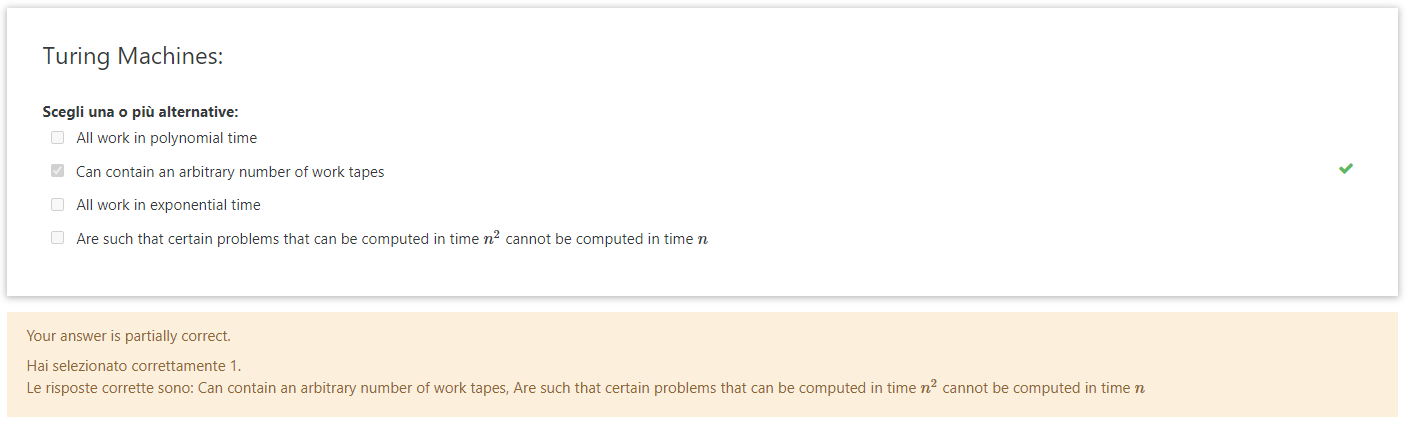
\includegraphics[scale=0.5]{figures/old/theory/4}}
% \end{figure}
%  \begin{figure}[H]
% \centerline{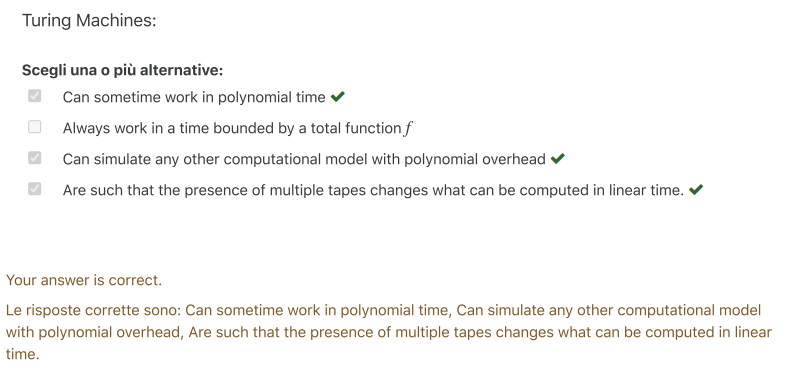
\includegraphics[scale=0.5]{figures/old/theory/5}}
% \end{figure}
%  \begin{figure}[H]
% \centerline{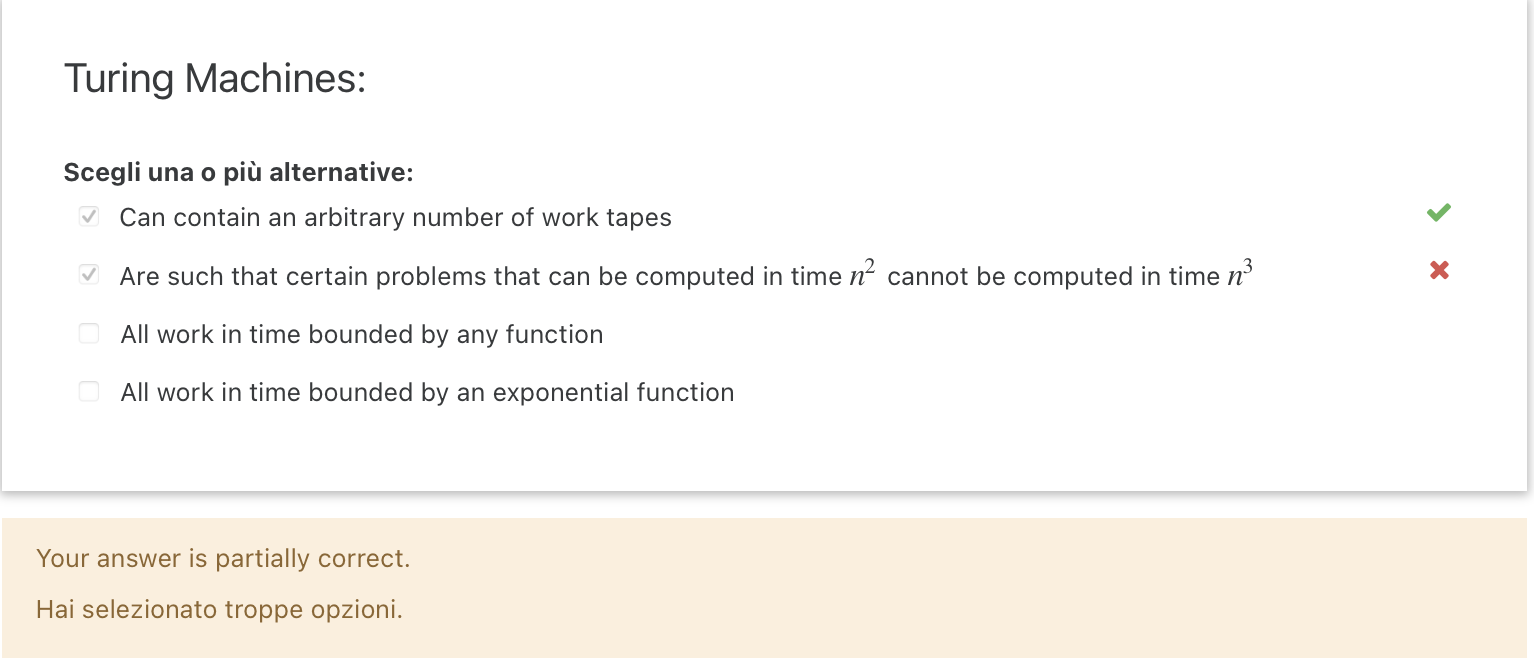
\includegraphics[scale=0.5]{figures/old/theory/6}}
% \end{figure}
%  \begin{figure}[H]
% \centerline{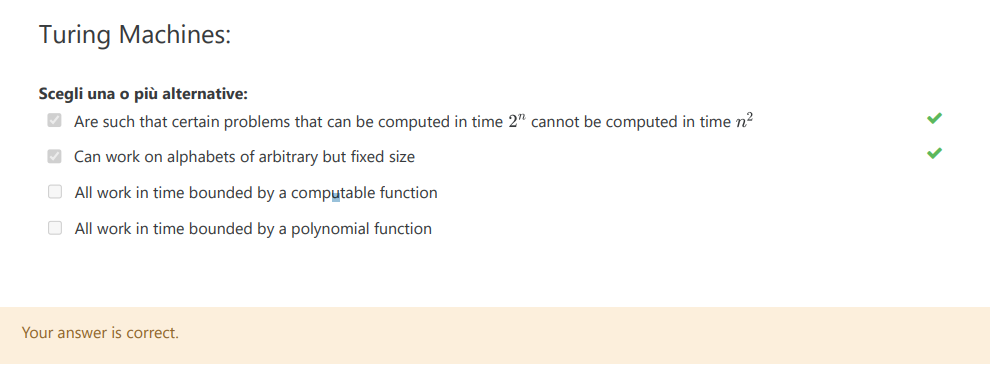
\includegraphics[scale=0.5]{figures/old/theory/7}}
% \end{figure}
%  \begin{figure}[H]
% \centerline{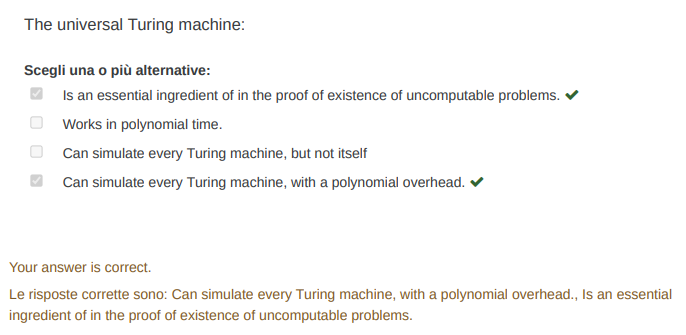
\includegraphics[scale=0.5]{figures/old/theory/8}}
% \end{figure}
%  \begin{figure}[H]
% \centerline{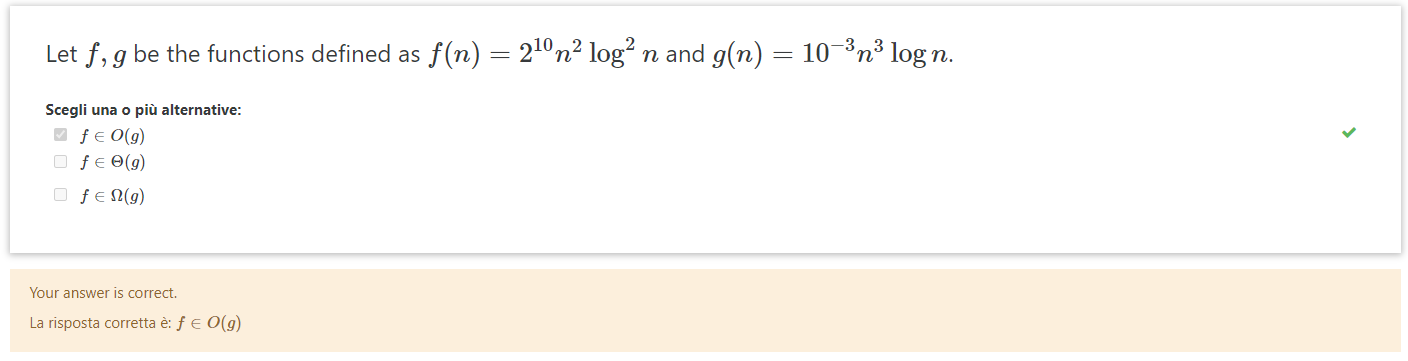
\includegraphics[scale=0.5]{figures/old/theory/9}}
% \end{figure}
%  \begin{figure}[H]
% \centerline{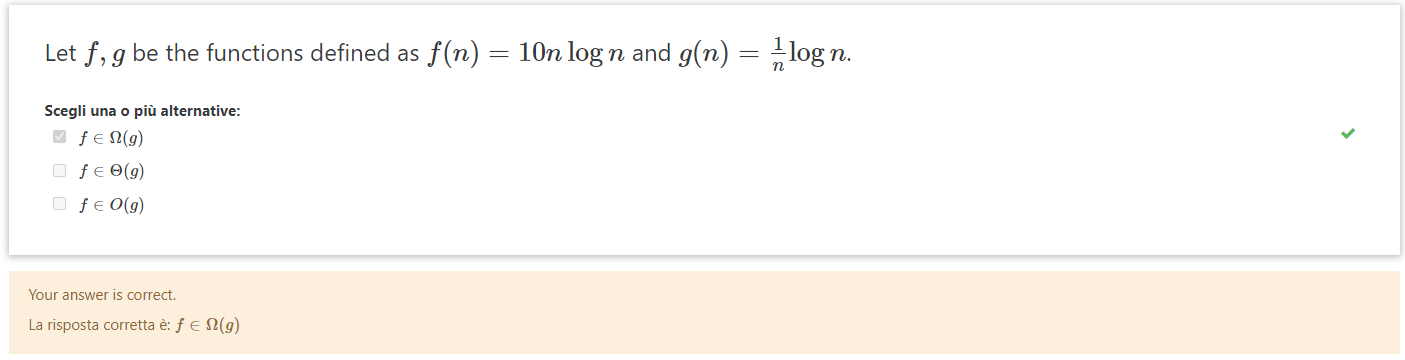
\includegraphics[scale=0.5]{figures/old/theory/10}}
% \end{figure}
%  \begin{figure}[H]
% \centerline{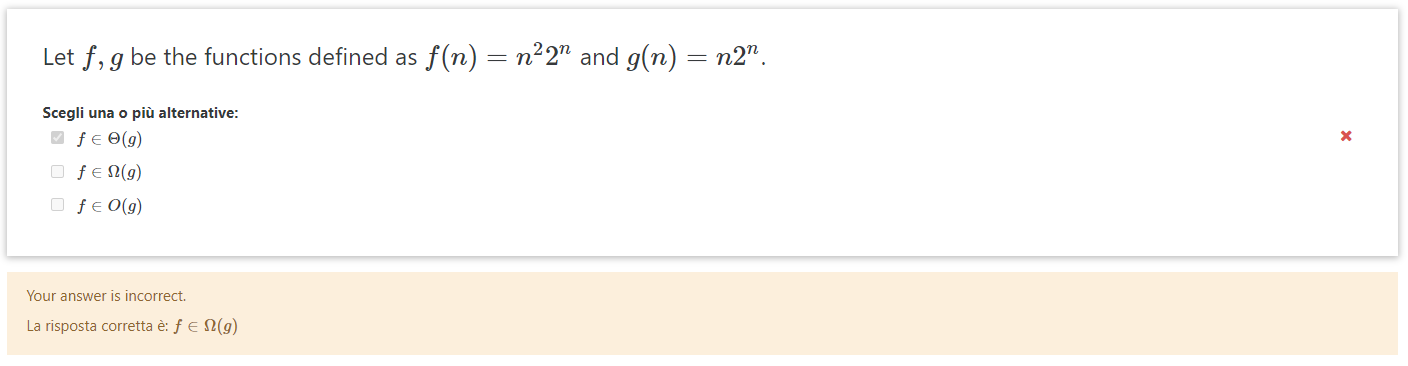
\includegraphics[scale=0.5]{figures/old/theory/11}}
% \end{figure}
%  \begin{figure}[H]
% \centerline{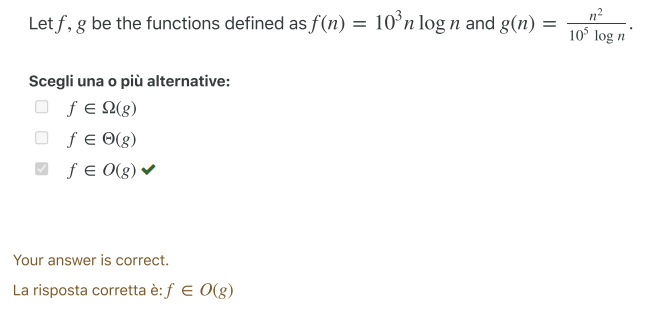
\includegraphics[scale=0.5]{figures/old/theory/12}}
% \end{figure}
%  \begin{figure}[H]
% \centerline{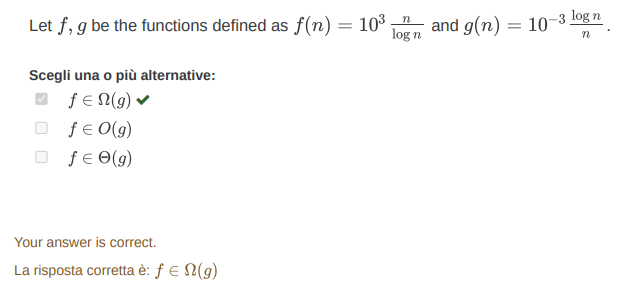
\includegraphics[scale=0.5]{figures/old/theory/13}}
% \end{figure}
%  \begin{figure}[H]
% \centerline{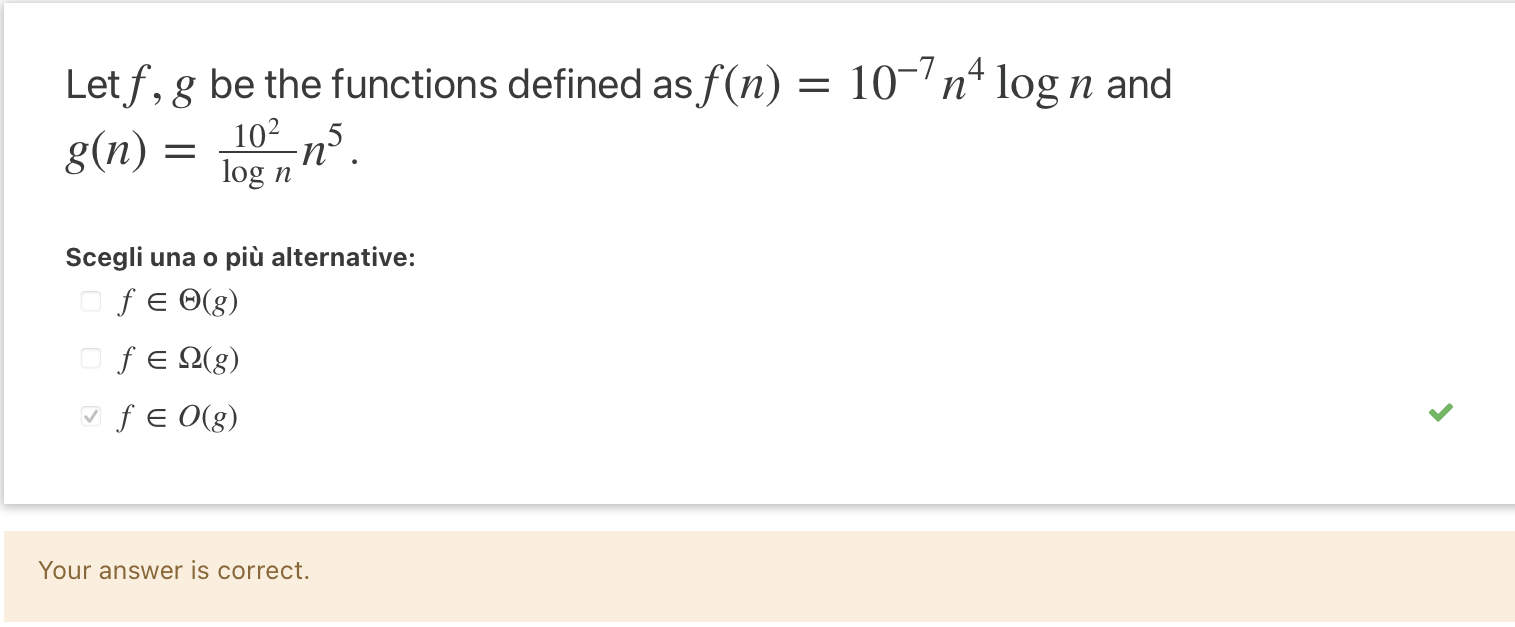
\includegraphics[scale=0.5]{figures/old/theory/14}}
% \end{figure}
%  \begin{figure}[H]
% \centerline{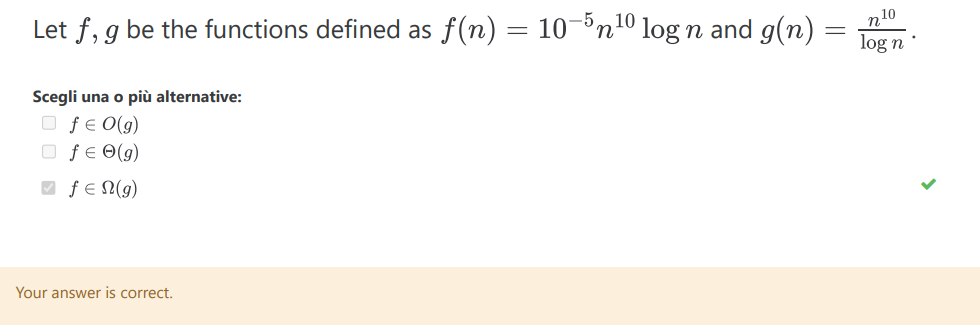
\includegraphics[scale=0.5]{figures/old/theory/15}}
% \end{figure}
%  \begin{figure}[H]
% \centerline{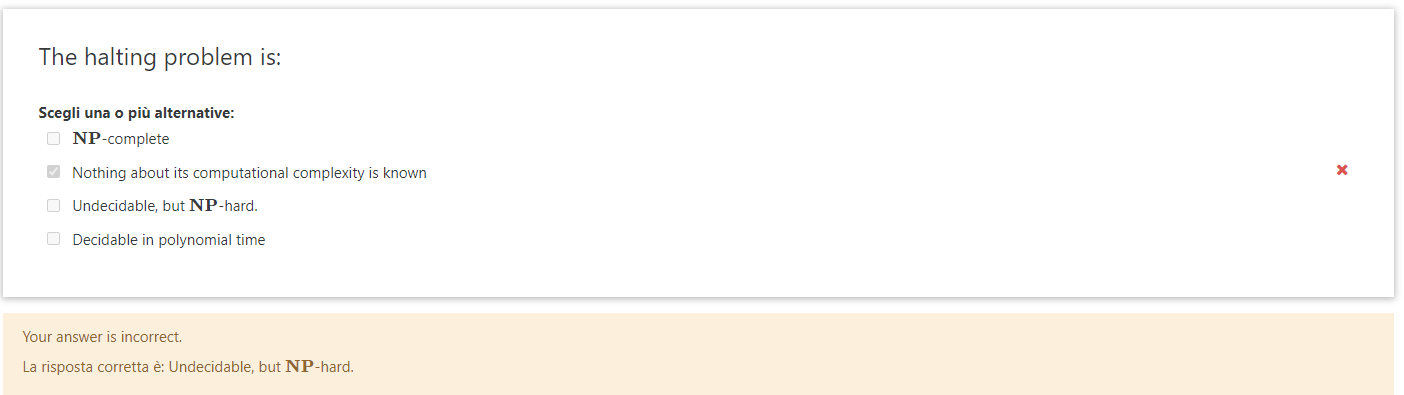
\includegraphics[scale=0.5]{figures/old/theory/16}}
% \end{figure}
%  \begin{figure}[H]
% \centerline{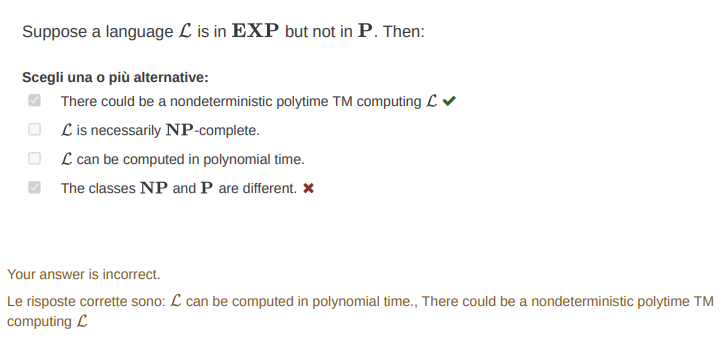
\includegraphics[scale=0.5]{figures/old/theory/17}}
% \end{figure}
%  \begin{figure}[H]
% \centerline{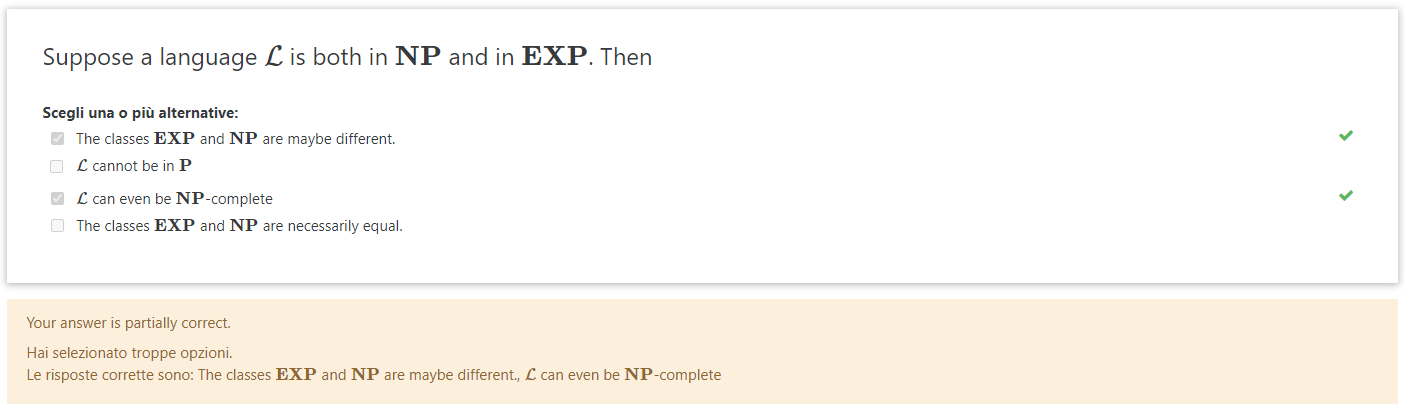
\includegraphics[scale=0.5]{figures/old/theory/18}}
% \end{figure}
%  \begin{figure}[H]
% \centerline{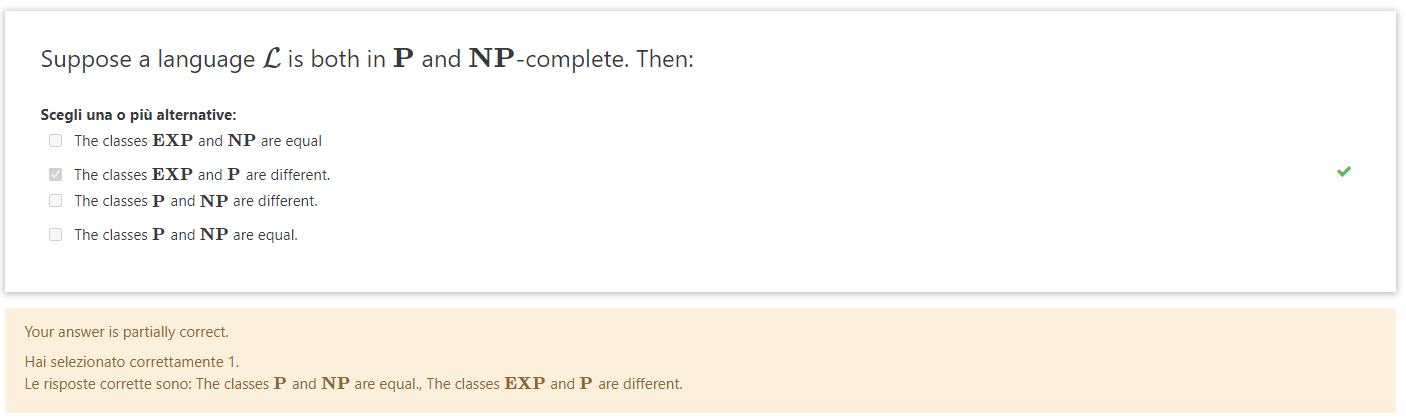
\includegraphics[scale=0.5]{figures/old/theory/19}}
% \end{figure}
%  \begin{figure}[H]
% \centerline{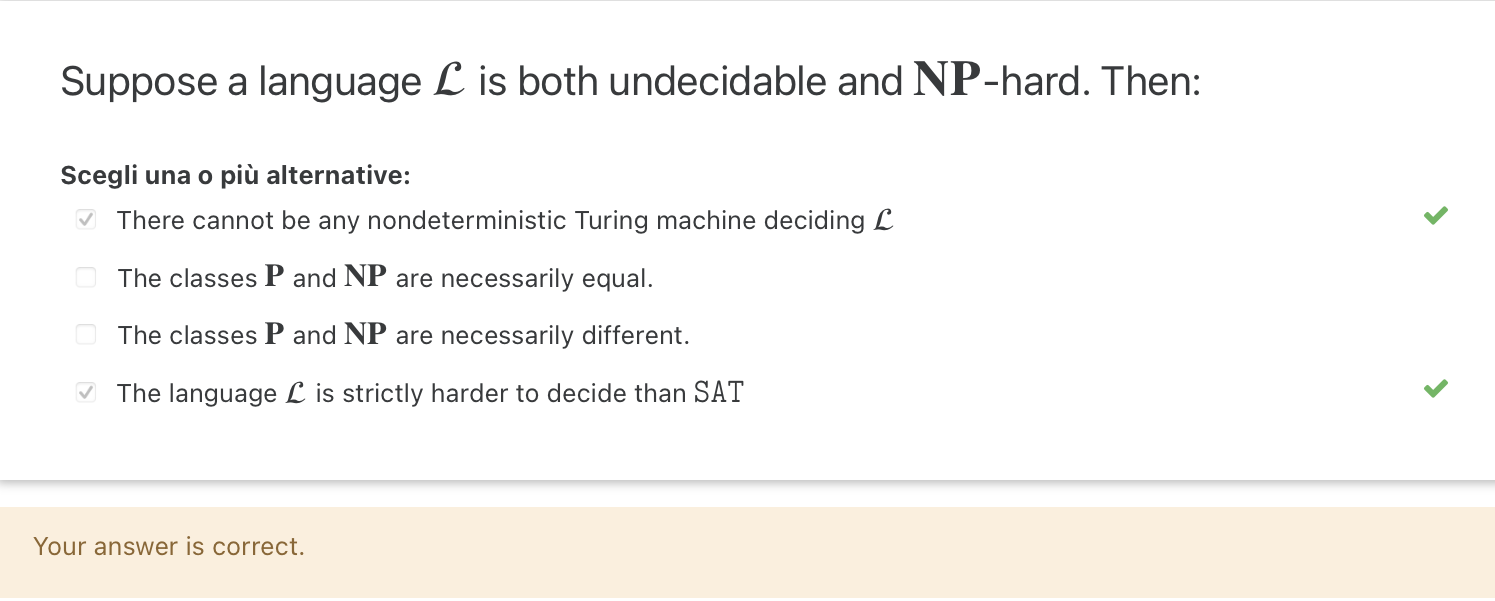
\includegraphics[scale=0.5]{figures/old/theory/20}}
% \end{figure}
%  \begin{figure}[H]
% \centerline{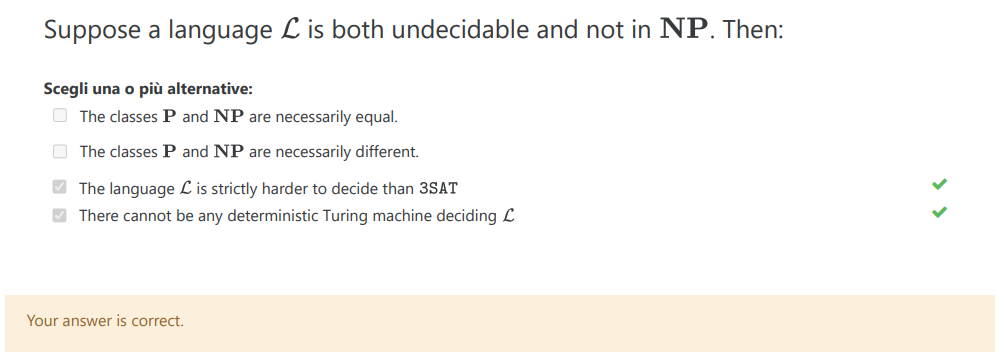
\includegraphics[scale=0.5]{figures/old/theory/21}}
% \end{figure}
%  \begin{figure}[H]
% \centerline{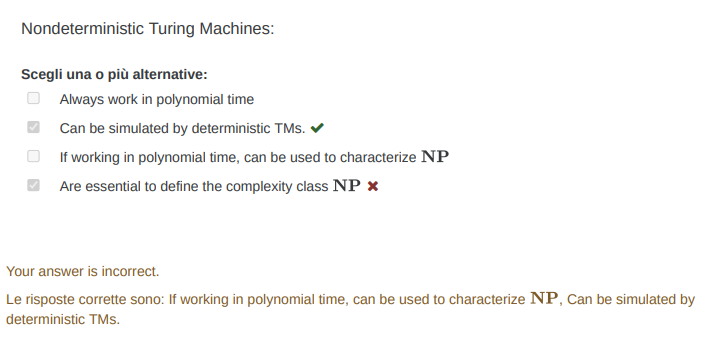
\includegraphics[scale=0.5]{figures/old/theory/22}}
% \end{figure}
%  \begin{figure}[H]
% \centerline{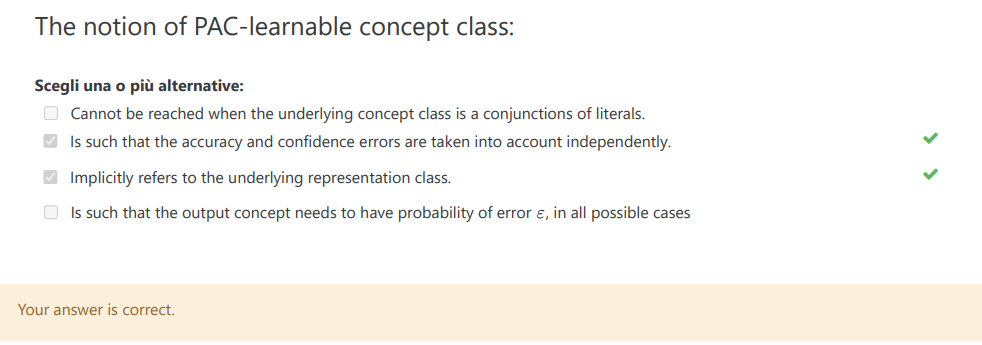
\includegraphics[scale=0.5]{figures/old/theory/23}}
% \end{figure}
%  \begin{figure}[H]
% \centerline{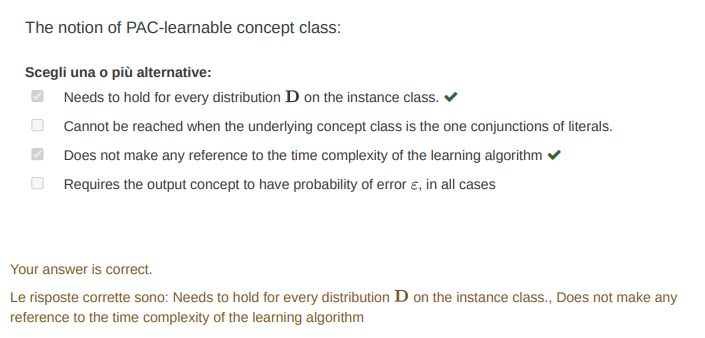
\includegraphics[scale=0.5]{figures/old/theory/24}}
% \end{figure}
%  \begin{figure}[H]
% \centerline{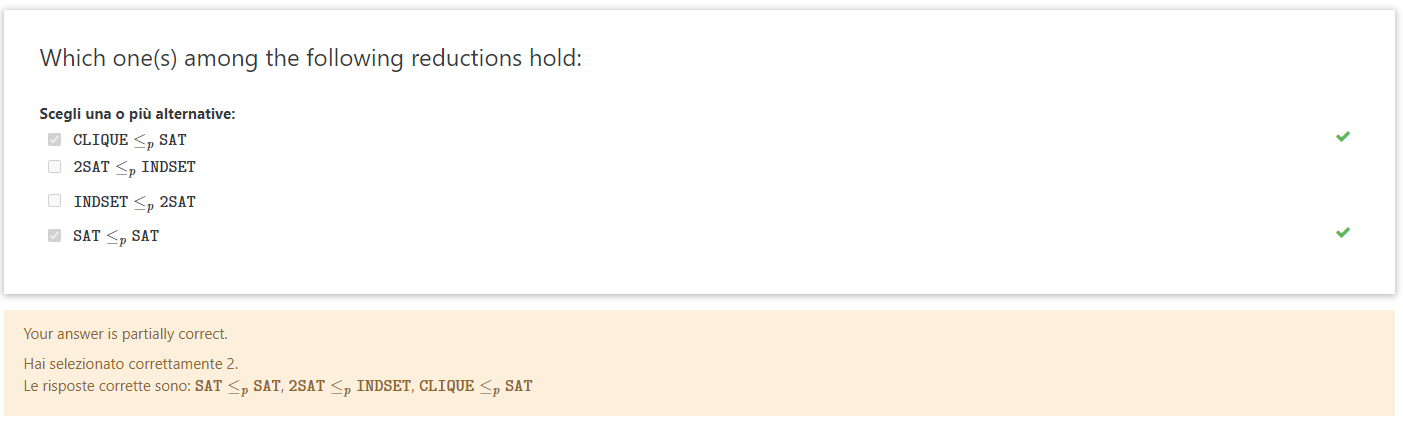
\includegraphics[scale=0.5]{figures/old/theory/25}}
% \end{figure}





\printbibliography[heading=bibintoc]

% back cover
% \includepdf[pages=2, fitpaper=true]{./kuleuven-template/covers.pdf}
\end{document}
